% ****** Start of file apssamp.tex ******
%
%   This file is part of the APS files in the REVTeX 4.1 distribution.
%   Version 4.1r of REVTeX, August 2010
%
\documentclass[reprint,%article
 %,
%superscriptaddress,
%groupedaddress,
%unsortedaddress,
%runinaddress,
%frontmatterverbose, 
%preprint,
%showpacs,preprintnumbers,
%nofootinbib,
%nobibnotes,
%bibnotes,
 amsmath,amssymb,
 aps,
%pra,
%prb,
%rmp,
%prstab,
%prstper,
%floatfix,
]{revtex4-1}

\usepackage{xcolor}

\usepackage{graphicx}% Include figure files
\usepackage{dcolumn}% Align table columns on decimal point
\usepackage{bm}% bold math
\usepackage{appendix}
\usepackage{subcaption}
%\usepackage{subfloat}
%\usepackage{hyperref}% add hypertext capabilities
%\usepackage[mathlines]{lineno}% Enable numbering of text and display math
%\linenumbers\relax % Commence numbering lines

%\usepackage[showframe,%Uncomment any one of the following lines to test 
%%scale=0.7, marginratio={1:1, 2:3}, ignoreall,% default settings
%%text={7in,10in},centering,
%%margin=1.5in,
%%total={6.5in,8.75in}, top=1.2in, left=0.9in, includefoot,
%%height=10in,a5paper,hmargin={3cm,0.8in},
%]{geometry}https://www.overleaf.com/project/5ba0361831a91c7b3990c0d7
 \usepackage{natbib}
 
\begin{document}

\preprint{APS/123-QED}

\title{DRAFT- Rotation Curve Fitting Model }% Force line breaks with \\
%\thanks{ Thanks Jesus}%

% Find out if Joe and Noah still want to be on this paper%

 

\author{Sophia Natalia Cisneros}
 \affiliation{ Department of Physics and Astronomy,  
 University of Denver.}
 % \email{sophia.cisneros@du.edu}
  \author{Richard Ott}%
 \email{rich.ott@EMAIL.com}
\affiliation{Something}%Tech dudes \textbackslash\textbackslash
%}
 \author{ Meagan Crowley}
\email{ }
\affiliation{NREL}%


\author{Zaneeyiah Brown}
\author{Landon Joyal}
\author{Roberto Real Rico}
\author{Marcus Paz}
\author{Elizabeth Gutierrez-Gutierrez}
\author{Amanda Livingston}
\author{Lily Castrellon}
\author{Zac Holland}
\author{ Phong Pham}
\author{Shanon Rubin}
\author{Aaron Ashley}
\author{Dillon Battaglia}
%\affiliation{UMass Boston% with \\
%&}%
%
%\affiliation{%
%University Denver
%}%

%\affiliation{%
%UC Davis
%
%%\\author{J.G. O'Brien}%
%\affiliation{%
%Wentworth Institute of Technology 
% 

 
\date{\today}% It is always \today, today,
             %  but any date may be explicitly specified
\begin{abstract}
{\color{teal}OPEN TO EDITS  }
The flat-rotation curve problem of spiral galaxies is generally resolved by the introduction of new physics.
 Dark Matter theories introduce new particles and Modified Newtonian Dynamics a new acceleration scale. In both paradigms,     Doppler shifted spectra     are interpreted by a Lorentz boost as  orbital velocities,  which diverge from the   expectations of Keplerian orbital velocities from luminous mass estimates. 
 We will instead view, excesses in shifted characteristic spectra  as relative gravitational frame effects due to our Milky Way. 
     Our   approach  employs  a new technique, but no new physics.  
 We compare in this paper  this new relative frame approach  on  the SPARC sample of 174 galaxies (Spitzer  Photometry and Accurate Rotation Curves) as  compared to MOdified Newtonian Dynamics (MOND) for the same  sample.  

\begin{description}
\item[Usage]
Secondary publications and information retrieval purposes.
\item[PACS numbers]
May be entered using the \verb+\pacs{#1}+ command.
\item[Structure]
You may use the \texttt{description} environment to structure your abstract;
use the optional argument of the \verb+\item+ command to give the category of each item. 
\end{description}
\end{abstract}

\pacs{Valid PACS appear here}% PACS, the Physics and Astronomy
                             % Classification Scheme.
%\keywords{Suggested keywords}%Use showkeys class option if keyword
                              %display desired
\maketitle

%\tableofcontents
%%%%%%NOTES TO DO
%%%make labels for figure axes. remove orange line through the data



%%%%%%
%%%%%%%%
%%%%%%
%%%%%%%
%%%%%%
%%%%%%
\section{Introduction  \label{sec:uno}}
 {\color{teal} \rule{\linewidth}{0.5mm} (Marcus UPDATE GRAPHS).}

 
 The flat-rotation curve  problem in spiral galaxies is one of the primary evidences for dark matter \cite{Rub},\cite{Bosma}.  
 The flat-rotation curve problem is viewed as the divergence of two proxies for mass, rotation velocities from Doppler shifted spectra increase substantially past the Keplerian estimates for rotations from observations of total light  ( see Fig.~\ref{fig:NGC2403}).
When   both observations are interpreted as  proxies for mass,  then there is clearly a    missing or ``dark'' matter problem. However    the primary 
 alternative to dark matter,   MOdified Newtonian Dynamics (MOND) \cite{Milgrom}, instead asks ``why is the luminous tail wagging the dark matter dog,  if dark matter dominates dynamics ?'' \cite{1999McGaugh}.
 
 
  MOND    interprets  excesses in rotation curve velocities,  above estimates from the luminous mass, as due to a changing acceleration scale   on the enormous distance scales of galaxies and groups of galaxies.    MOND    focuses on   the   ``remarkably tight empirical correlations between the observed mass distribution and the corresponding dynamics.'' \cite{McGaugh_2014}. Using this approach, MOND is remarkably successful in fitting the same galaxy rotation curves as dark matter models, but using only estimates of the luminous mass, and an estimate of the new acceleration scale\cite{McGaugh2016RAR}. 
  
  
However, both theories share certain similarities. First,   dark matter and MOND theories interpret observed Doppler shifted spectra  as entirely due to relative motion. Secondly,  both require new physics. Dark matter models require galaxies to grow in    dark matter halos, and in simulations this does not lead to realistic galaxies \cite{de_Blok_2010}.  MOND requires modifications to standard gravity theory. 

What we will present here is  a new Rotation Curve Fitting Model (RCFM),  a heuristic  extension of  MONDian reasoning into a relativistic regime. We   transition the MONDian concept of  a changing gravitational acceleration scale,   to  the concept of relative curvature.  We use a  relative frame picture  where relative galaxy curvatures  are always considered with respect to a Milky Way baryon model, as a function of radius. 
Like MOND, the RCFM posits that the luminous mass is the only mass. Unlike MOND, it reproduces ``flat'' rotation curves
 without modifying Einstein's gravity. 
   We assume   photometric estimates of total light are Lorentz scalars, given a good distance estimate, and that Doppler shifted spectra form a part of a 4-vector. 
 
 
 The RCFM interprets excesses Doppler shifted spectra  (above estimates from baryonic mass) not as physical velocities.  We use Lorentz type transformations to relate relative galaxies by their field frames, quantified by the Schwarzschild gravitational redshifts in the weak field limit.  In this paper,    we  efficiently reproduce  the flat-rotation curves of a large sample of diverse galaxies,  with no new physics.
 Previous investigations of gravitational redshifts in the flat-rotation curve problem   used  Galilean differences of gravitational redshifts to relate galaxy frames at the large $r$ limit of the data \cite{MTW}.
 
 
  
 Dark matter is   involved in many places in the concordance model of cosmology,     $\lambda$CDM. In  this paper, we   address only the flat-rotation curve problem.      We do not present a fundamental derivation of our fitting formulae, but only  show  that there exist a  class of  Lorentz-type transformations  which compactly  reproduces galaxy rotation curves   with no   new physics.    We demonstrate RCFM  fits on the SPARC\cite{2016Lelli} galaxy sample   reported previously by     MOND \cite{McGaugh2016RAR}. 
   
 
 
  
  
  
  
 \begin{figure}[h!]
%\scalebox{0.25075}%
      \centering
      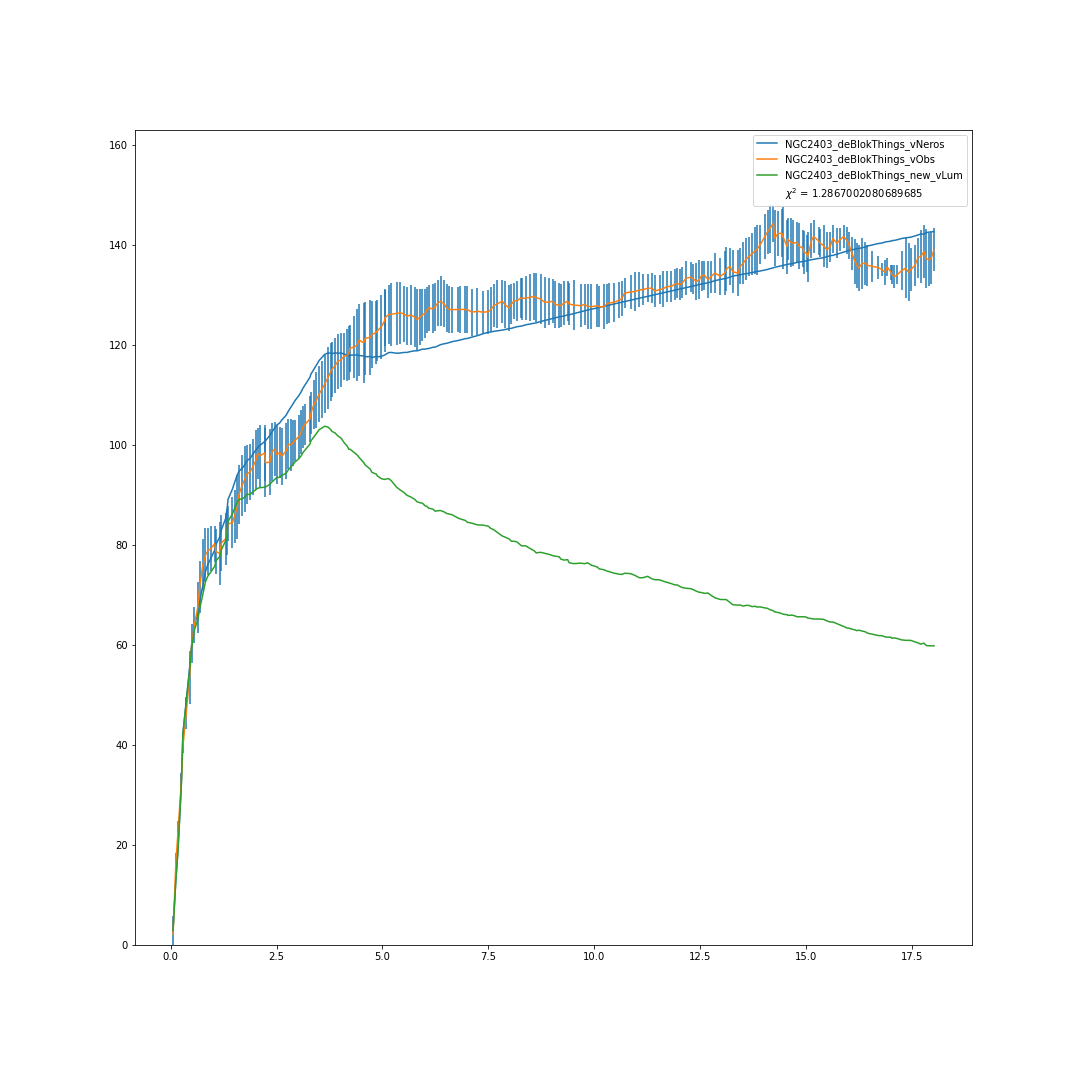
\includegraphics[width=\linewidth]{NGC2403_deBlokThings_XueSofue}
      \caption{Rotation Curve of NGC 2403 \cite{Blok1},  Rotation curve data points blue dots with  error bars, expected velocity from baryons estimated by the green line. }
      \label{fig:NGC2403}
  \end{figure}
  
       
  
 {\color{teal} edit when sections gelled}\\
 {\color{teal} \rule{\linewidth}{0.5mm}}
 
This paper  is organized as follows;
{\bf Section 2} describes the heuristic  fitting formula, 
{\bf Section 3} describes fits and probabilities on the
 SPARC galaxy data set versus    the Milky Way from  XueSofue (CITE-xuesofuerubin), 
 {\bf Section 4} describes fixing the free parameter,   and   
{\bf Section 5}  presents conclusions.     
  

   
 
   
 
 
 
  
 
%%%%%%
%%%%%%%%
%%%%%%
%%%%%%%
%%%%%%
%%%%%%
\section{  heuristic picture and fitting formulae  \label{sec:dos}}
 {\color{teal} \rule{\linewidth}{0.5mm}}
 
 {\color{teal}Sofia - still editing}
 {\color{teal} \rule{\linewidth}{0.5mm}}
 
\begin{figure}[h!]
     \centering
     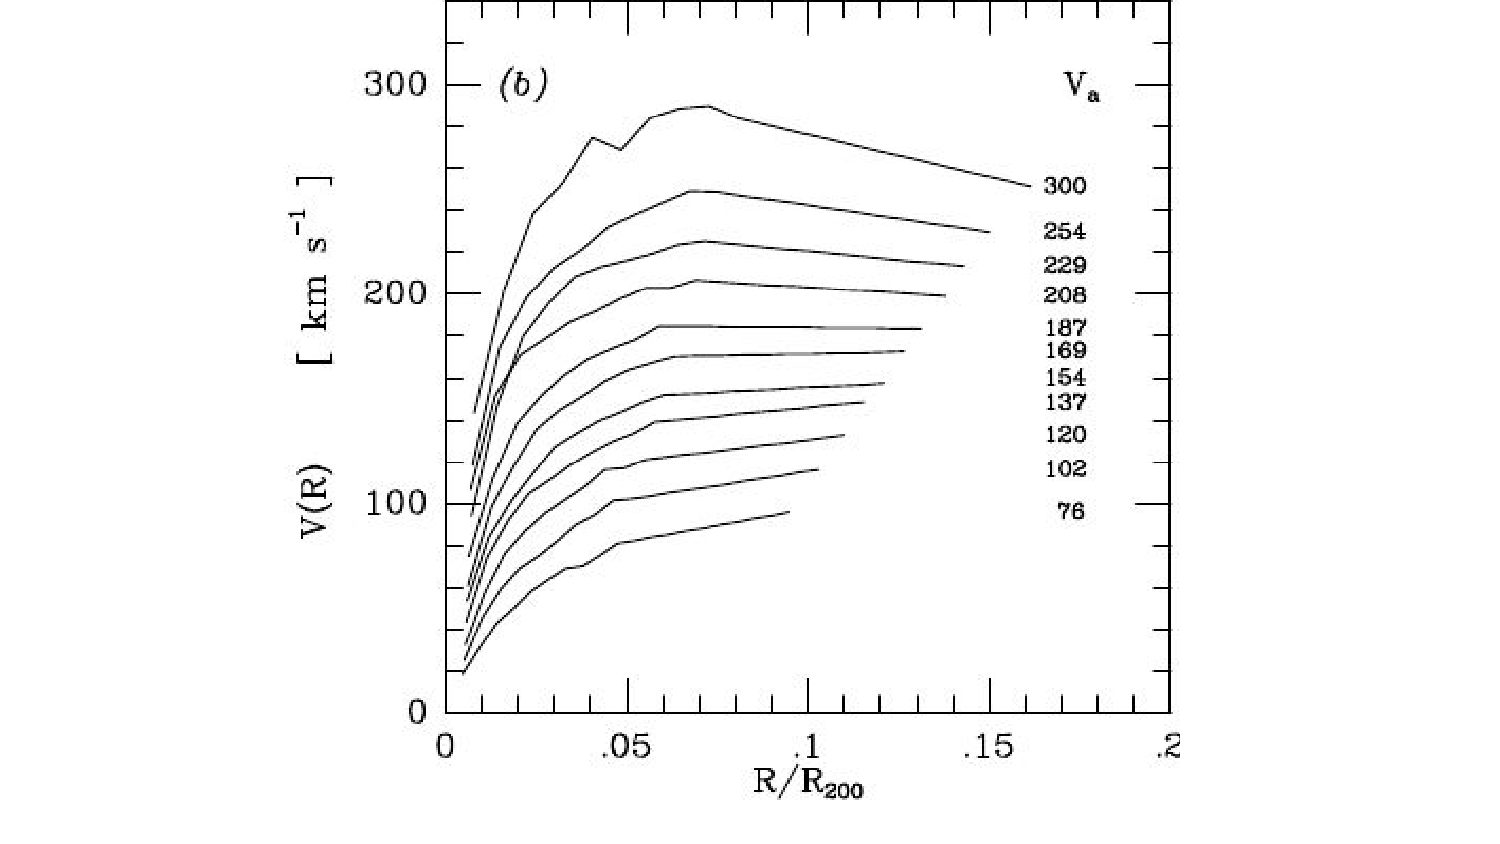
\includegraphics[width=\linewidth]{URC}
     \caption{Universal Rotation Curve spectrum, Used with permission from Ref.\citep{salucci}}
     \label{fig:URC}
\end{figure}
The strange correlation between luminous and  dark matter  can be seen in the Universal Rotation Curve spectrum of 1,100 rotation curves Fig.~\ref{fig:URC} normalized by scale-length, which inflect about the rotation curves for galaxies on the same size order of luminous mass as  the Milky Way in baryonic mass. Galaxies larger than the Milky Way occupy the upper portion of rotation curves which inflect down (albeit not in a Keplerian manner), and those galaxies smaller than the Milky Way inflect up.  This leads to fine-tuning problems in  dark matter theory, where
   galaxies smaller than the Milky Way require proportionally larger  dark matter halos than      galaxies larger than the Milky Way.   We interpret this as a frame dependent effect in the observations of Doppler shifted spectra. We will   transition the MONDian idea of changing acceleration scales  to a relative galaxy-frame picture, interpreting excesses in the rotation curve velocities at the level of the observed spectra. 
 

 \subsection{Rindler's standard of rest}
 {\color{teal} \rule{\linewidth}{0.5mm}}
 
{\color{teal} \rule{\linewidth}{0.5mm}}
 
 {\color{teal}Sofia - still editing}
 {\color{teal} \rule{\linewidth}{0.5mm}}
 
The first building block of the rotation curve fitting model (RCFM) presented here comes from an observation from W.    Rindler,    ``that the center of each galaxy provides a basic local standard of nonacceleration, ... and so then can be treated like a local inertial frame relative to our own center.''\cite{rindler2013essential}. 
 We will use this concept  to characterize excesses in Doppler shifted spectra within a relative galaxy mapping formalism.    
 
 Schwarzschild gravitational redshifts  
 
     \begin{equation}
       \frac{\omega_1}{\omega_2}  =\sqrt{\frac{g_{tt}(r)|_{P2}}{g_{tt}(r)|_{P1}}} =\sqrt{\frac{|\xi^t\xi_{t}|_{P2}}{|\xi^t\xi_{t}|_{P1}}}. 
      \label{eq:grav}
    \end{equation}
    
  relate    frames   at   $P1$ and $P2$ within one  Killing vector field $\xi^t$ by the ratio of the emitted and received frequencies \cite{Wald}.  
  Schwarzschild clock  terms $g_{tt}(r)$ defining the timelike Killing field      are 
   
  \begin{equation}
      g_{tt}(r)= -( 1 - 2\Phi(r)/ c^2), 
      \label{clocktime}
  \end{equation} 
  
for $\Phi (r)$ 
the Newtonian  gravitational potentials, $r$  the radius from the galactic center, and $c$   the vacuum light speed, in the weak field limit  in Boyer-Lindquist coordinates \cite{Hartle}. 
  
To map two galaxies onto each other, we extend   Eq.~\ref{eq:grav} to   mapping two separate Killing manifolds (vis galaxies) onto one another  one-to-one in radius. We do this by synchronizing the 
 clock terms  $g_{tt}$,  at the level of  the   $\Phi (r)$. 
 
 To synchronize $\Phi (r)$ terms, we   integrate    gravitational potentials from   $\Phi = 0$ at the  smallest $r$,  to some positive finite value at the large $r$ limit
    
  
 
    \begin{equation}
     | \Phi  (r) |= \left| \int^{R\to \infty}_{r} \vec{F_r}\cdot\vec{dr} \right|.
      \label{eq:Newt2}
      \end{equation}
 
   The Newtonian potentials integrated in this way  represent clocks compared from the same standard of rest, and   obey the central force law for test particles moving in circular orbits

\begin{equation}
 \frac{\partial \Phi_{lum}(r)}{\partial r}    =\frac{v_{lum}(r)^2}{r},  
    \label{zoochance1}
\end{equation}

 and Poisson's equation
 
\begin{equation}
\nabla^2 \Phi_{lum} (r) = 4\pi G \rho (r).   
    \label{whatsgood}
\end{equation}

 
 
   Newtonian gravitational potentials $\Phi(r)$  are usually integrated in the opposite way, from the large $r$ limit assumed to be the zero of the 
     potential. This is  an implicit assumption that all galaxies are embedded in the same flat spacetime. Since we have no clear notion of the external embedding environments of galaxies (Hubble flow, dark energy content, curvature of the universe, etc), and since we need to syncronoize clocks,  we compare the 
   $\Phi(r)$ from where we know they all have the same curvature (at $r=0$).
   
    
 
Schwarzschild is a spherically symmetric spacetime, so in the plane of the galaxy disk the geometries are isomorphic. 

 \subsection{Universal Rotation Curve }

 {\color{teal} \rule{\linewidth}{0.5mm}}
 
{\color{teal} \rule{\linewidth}{0.5mm}}
 
 {\color{teal}Sofia - still editing}
 {\color{teal} \rule{\linewidth}{0.5mm}}
 
 The second important building block of the new rotation curve interpretation  presented here   is from      the Universal Rotation Curve (URC) discovered by   Persic and Salucci and Rubin \cite{salucci}, \cite{Persic},  \cite{1978Rubin}.  The URC is  a collection of  1,100 galaxy rotation curves   plotted on the same   axes  and normalized by the  respective galaxy scale-lengths.  As can be seen   in Fig.~\ref{fig:URC},    
 the spectrum   inflects about   the assumed rotation curve of our   Milky Way.  Interpreted through a dark matter lens, the URC requires  
   galaxies smaller than the Milky Way to be more successful at accretion of    dark matter halos, than those    larger than the Milky Way.
   This means,  smaller masses tend to be   proportionally more successful at assembly of  larger dark matter halos counter to    classical gravitation theory.    In the simpler RCFM perspective,  the URC spectrum    represents the frame dependence of our Milky Way imposed onto the spectra  we receive  from external galaxies.  
 
  
 The standard dark matter rotation curve formula is

 \begin{equation}
v_{obs}^2 (r)=  v^2_{lum}(r) +  v^2_{dm}(r),  
\label{eq:zonte1}
\end{equation} 

where  the dark matter term $v_{dm}$ makes up the difference between velocities from Doppler shifted spectra  $v_{obs}$ and those from observations of total light associated with baryonic mass $v_{lum}$. Velocities are added in quadrature to reflect a mass sum   by Eq.~\ref{zoochance1}.


 
To re-phrase reported rotation curve velocities $v_{obs}$ in Eq.~\ref{eq:zonte1}, we look at how 
observations of Doppler shifted spectra $\omega'$ are    interpreted   as  relative    frame velocities  by the  Lorentz   Doppler shift formula 
 
 \begin{equation}
 \frac{v_{obs}}{c}=
\frac{  \frac{\omega'(r)}{\omega_o} -  \frac{\omega_o}{\omega'(r)}  }{  \frac{\omega'(r)}{\omega_o}  +  \frac{\omega_o}{\omega'(r)} } . 
\label{eq:modelLumA}
\end{equation} 
 
We will modify
the rotation curve formula in Eq.~\ref{eq:zonte1} by replacing the dark matter term with a product  of a curvature ratio $\kappa^2$ and two Lorentz-type transforms     $v_1$ and $v_2$ between galaxies,   

\begin{equation}
v_{rcfm}^2 =  v_{lum}^2+\alpha \kappa^2 v_{1}v_{2}, 
\label{eq:zonteLCM}
\end{equation}  

 where all terms   are a function of $r$ except the model's free fitting parameter $\alpha$. 
The  RCFM  prediction $v_{rcfm}$ is then fitted to the observations in $v_{obs}$,   with the     parameter $\alpha$ being free, and single valued for each galaxy    fitted. 

Terms in $ \kappa^2 v_{1}v_{2}$ are   maps between the galaxy being observed and the Milky Way, and so we   assume a static MW baryon profile. In this paper we fit the SPARC sample to  a few different such MW models. 



 Terms in $\kappa$ 
 represent a  
curvature ratio  

 \begin{equation}
\kappa(r)=\frac{\Phi_{gal}(r)}{\Phi_{mw}(r)}.  
\label{eq:kappa2}  
\end{equation}  
 
 
Terms in $v_1$   will  map between the two galaxies (sending and receiving the light signal) one-to-one in $r$, and $v_2$ terms will map from the 2-frame of the first mapping back to the flat frames where observations are made. That this second step is necessary is evidenced by the fact that we do not require dark matter to reproduce the Solar System rotation curve.  

 The mapping terms will be constructed based on the 
 Lorentz exponentials in the   standard flat spacetime  Minkowski boost, 
 where   the  hyperbolic  transformation  

     \begin{equation}
         \frac{v}{c} = \tanh \zeta = \frac{e^\zeta - e^{-\zeta}}{e^\zeta + e^{-\zeta}}   
         \label{boost}
     \end{equation} 

 through a rapidity hyperbolic angle $\zeta$ relates sending and receiving frames by  the
    Lorentz exponential term  $e^\zeta = \omega'(r) /\omega_o$. In Special Relativity the frames are   symmetric between the sender and receiver. However, to introduce gravity is to pin the frames, so for consistency we will interpret the general Lorentz exponential object as the ratio of the receiving frame frequency over the   sending frame frequency.  
 
For the $v_1$ term then, we compose a   Lorentz exponential term  in galaxy redshifts
 
     \begin{equation}
     e^{\gamma}(r)=  \frac{\omega_{MW}}{\omega_{gal}}  =\sqrt{\frac{g_{tt}(r)|_{gal}}{g_{tt}(r)|_{MW}}} =\sqrt{\frac{|\xi^t\xi_{t}|_{gal}}{|\xi^t\xi_{t}|_{MW}}}. 
      \label{eq:gravRS}
    \end{equation}
 evaluated at the same $r$ in different manifolds. 
   
 
The  second transform will map  from the 2-curved frames, to the 2-flat frames  where we make observations.

We identify the flat frame Lorentz exponential with the Doppler shifts $\omega'_{lum}$ expected for      Keplerian rotation velocities $v_{lum}$,   calculated from  observations of total light, Eq.~\ref{eq:zonte3},

\begin{equation}
    e^{\eta}(r)=\omega'_{lum}(r)/\omega_o.  
    \label{eq:flat}
  \end{equation} 
  
 This approach is suggested by   the fact that dark matter is not required to reproduce the rotation curve in the  solar system.  


To map from the  2-galaxy frame represented by $ e^{\gamma}$ to the $ e^{\eta}$, we define the last   Lorentz exponential term
 

\begin{equation}
    e^{2\xi}=   e^{\eta-\gamma}  .
\end{equation}

 
 
 
 The second transformation  $v_2$ maps the 2-frame for the galaxies into the flat frames where we make observations. 



In what follows, we will explore the hyperbolic function space of  Rindler's accelerated coordinates to map between galaxies, but all transformations will be based upon the same exponential terms identified with the field frames.
 we find a set of ($4$ or $5$??) composite $v_1 v_2$ functions as described in Table~\ref{tab:my_label}.
{\color{pink} \rule{\linewidth}{0.5mm}}


  
  The transformation from this curved 2-frame map to the flat frames is parametrized as 
  
   
  
  \begin{equation}
\frac{v_{2} }{c}=  \coth (fc),
\label{eq:hyperbolico}
\end{equation}


%%%%%%
%%%%%
%%%
%%
%
%%%%%%


  
%%%%%%
%%%%%%%
%%%%%%
%%%%%%
\section{Fits and probabilities on  the SPARC data set  }
 {\color{red} \rule{\linewidth}{0.5mm}}
 
 {\color{red}Meagan or Rich - EDITS}
 {\color{red} \rule{\linewidth}{0.5mm}}
 
  Note,  population synthesis modeling  is an under-constrained field  precisely because the measurement of Doppler shifted spectra did not constrain $v_{lum}$, but rather introduced    an   new quantity of gravitating mass. 
 
    
However, the question  asked by S. McGaugh (CITE) as to why  ``the   baryonic tail wags the dark matter dog.''can not be answered by dark matter theory alone. 



We transition the idea of excesses in Doppler shifted spectra from a  pure kinematic interpretation, in which terms in  $v_{obs}$ above estimates for  $v_{lum}$ represent real, orbital motions, to a regime in which the excesses in $\omega'$ represent.
  relative gravitational redshifts between the extended gravitational  frames of  galaxies. 
 The baryonic mass models reported in any rotation curve study are only as good as    as the distance estimate, so to train the model's free parameter we select a subset of galaxies who have Cepheid or Tip of the Red Giant Branch distance measurements.  When the free parameter is fixed to a constant value, we will then run on the entire SPARC data set, with the exception of 20-30 galaxies where Lelli et all 2016 excluded those galaxies which have an inclination greater than $85^o$ as impossible to constrain a proper surface brightness profile, and those at inclinations less than $35^o$ as being impossible to accurately report line of sight Doppler shifts.   
 
 We fit the SPARC sample of Spitzer Photometry and Accurate Rotation Curves for 174 galaxies  \cite{2016Lelli} wiht the RCFM presented here. 
We compare results with the work from MOND and RAR spanning  \citet{McGaugh_2014}- \citet{Li_2018}. 
  
 
%%%%%%
%%%%%%%%
%%%%%%
%%%%%%%
%%%%%%
%%%%%%
\subsection{Milky Way}
{\color{red}Choose a fixed MW in this paper. }

{\color{red} \rule{\linewidth}{0.5mm}}



IN \cite{Li2016ModellingMD} the bulge is more like Sofue. Not flat like McGaugh. 
To understand why. 
``using the recently released Gaia billion-star map8
, we propose a
Galactic disk mass distribution model which is based on the star density distribution
rather than the brightness and mass-to-light ratio. ''
TROUBLE: ``we obtain a flat rotation curve
which reproduces the key observed features with no need for a dark halo''.

\begin{figure*}
    \centering
    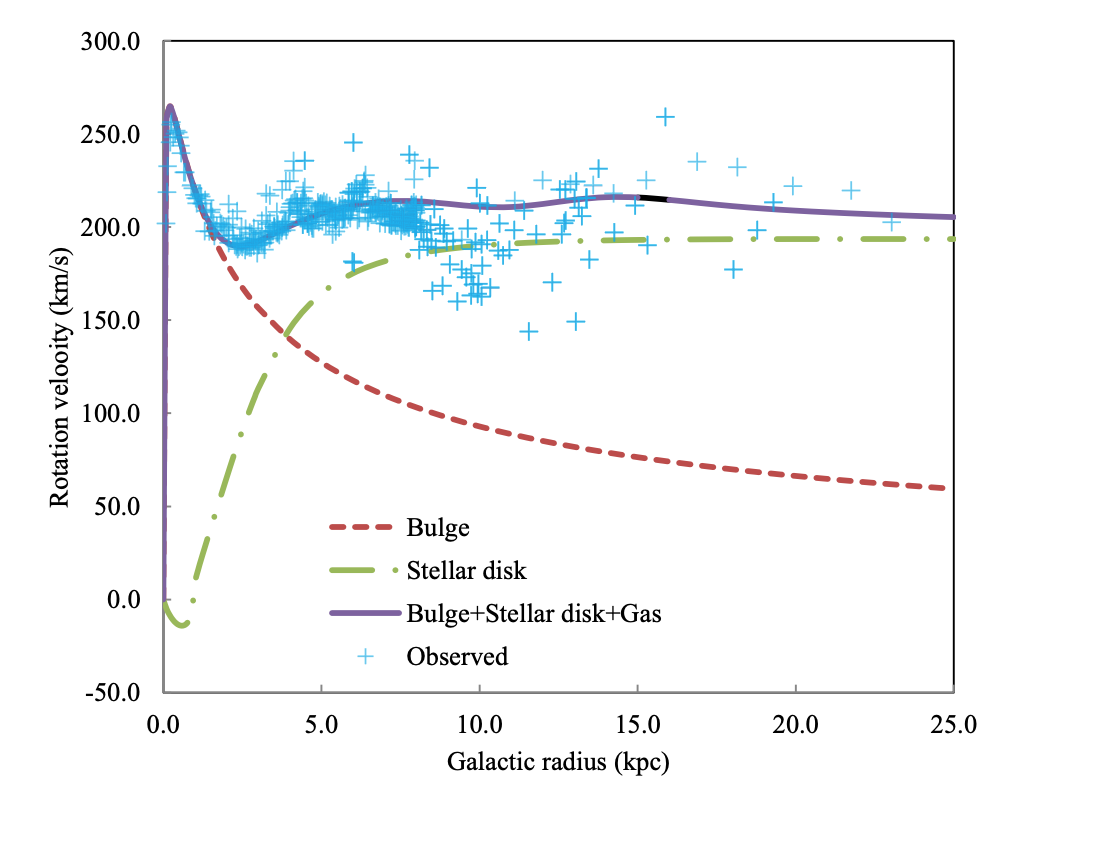
\includegraphics{MW_Enbang_Li}
    \caption{Enbang Li \cite{Li2016ModellingMD}}
    \label{fig:my_label}
\end{figure*}

\subsection{MOND Comparisons}


 In MOND,  classical gravity is transitioned to  a paradigm where the luminous mass is the only mass  but    the acceleration scale of gravity as represented by  Newton's  constant $G$ changes. This is an  interesting    question   on the enormous distance scales of spiral galaxies and larger structures, and we make a semi-relativistic extension of MOND 
 by considering relative curvatures with respect to the Milky Way. 
 \subsection{Sample}
 SPARC sample we test in this paper.   Relative galaxy curvatures have previously been   obviated in this context by Galilean subtraction of   gravitational red-shifts at the    limit of the data  \citep{MTW}. We instead use a 4-vector formalism to consider relative redshifts.  

 

 All terms in $\Phi(r)$ used in this paper  are   those reported in   the SPARC data base, from observations of total light, including the gas halo, stellar bulge and  stellar disk, 
 
  \begin{equation}
v_{lum}^2 (r)= \gamma_b v_{bulge}^2(r) +  \gamma_d v_{disk}^2(r) + v_{gas}^2(r),  
\label{eq:zonte3}
\end{equation} 
 
where the  $\gamma_i$  are  mass-to-light ratios of the stellar disk and bulge.   The    bulge and disk mass-to-light ratios are allowed to vary freely, though the average values are within stated criteria   \cite{2016Lelli} of $\pm 20\%$. The gas fractions (HI scaled for Helium abundance) are fixed though addition of molecular gas could increase mass fractions in the inner kiloparsec of a galaxy. 



 

 
\section{Free parameter fix }
 


This section shows some example fits from SPARC galaxies compared to different data and  Luminous mass models, to demonstrate how small changes in the   assumed  luminous mass model creates significant changes in the RC inflection at large radii. 
While error    estimates have not been standardized across the field~\citep{Blok,Gent,Toky},     one can reliably   compare fits to the same data with the same reported errors. The     reduced $\chi^2_r$ values printed on each graph, but goodness of fit can also be visually appraised.  
 
 \begin{figure}[h]
\begin{subfigure}{.5\textwidth}
  \centering
  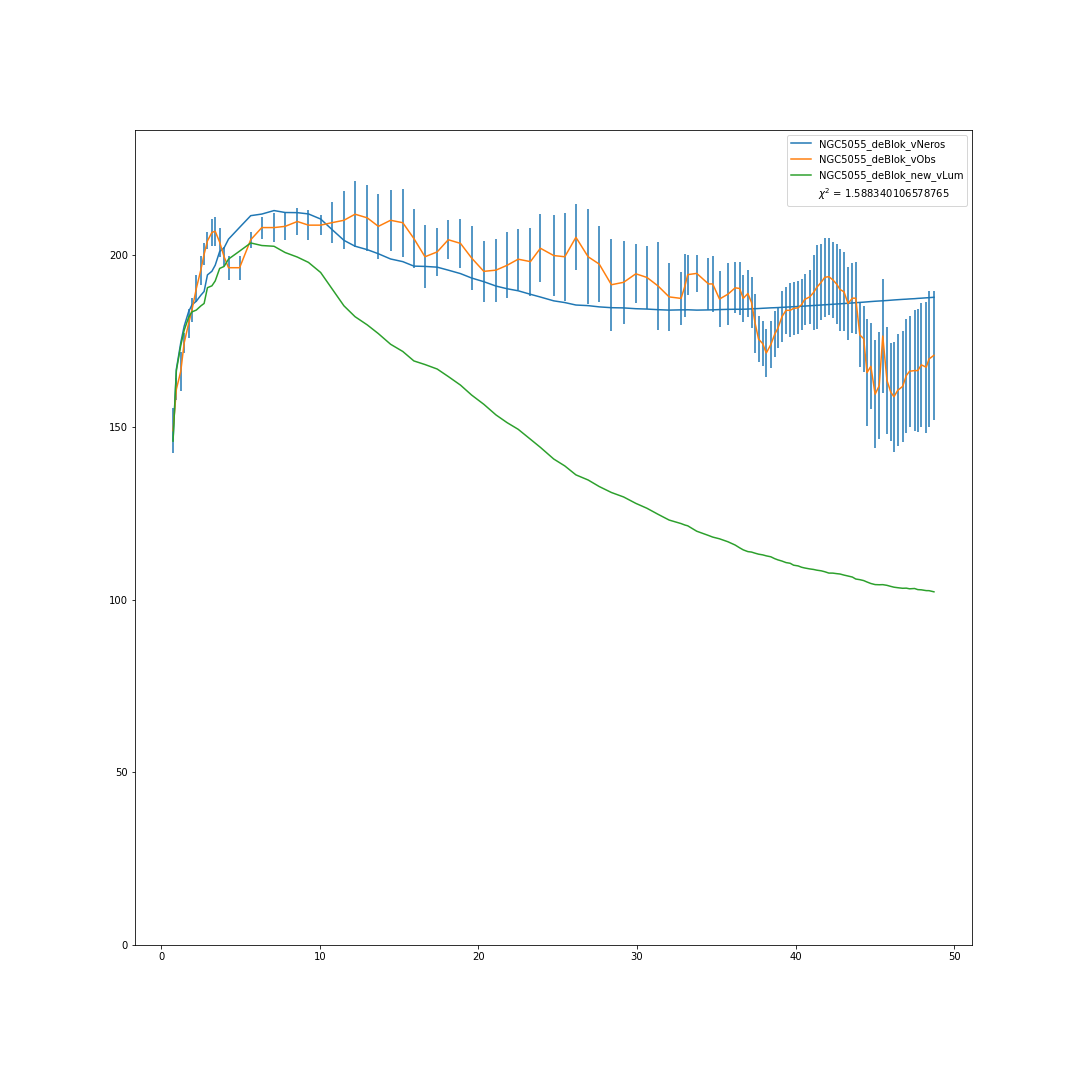
\includegraphics[width=.8\linewidth]{NGC5055_deBlok_XueSofue}
  \caption{deBlok\cite{Blok1}}
  \label{fig:sfig1}
\end{subfigure}%
\begin{subfigure}{.5\textwidth}
  \centering
  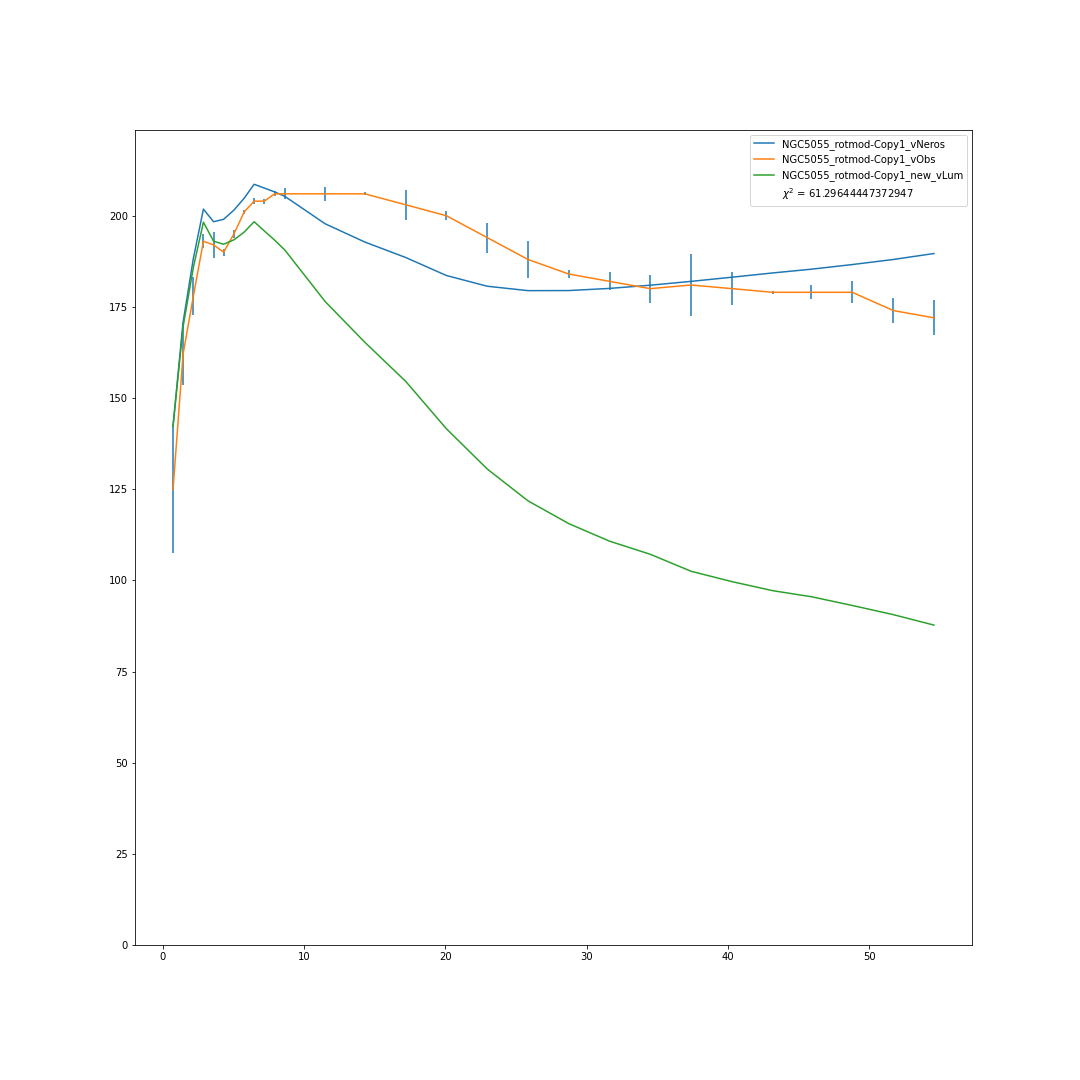
\includegraphics[width=.8\linewidth]{NGC5055_rotmod-Copy1_XueSofue}
  \caption{SPARC\cite{2016Lelli}}
  \label{fig:sfig2}
\end{subfigure}
\begin{subfigure}{.5\textwidth}
  \centering
  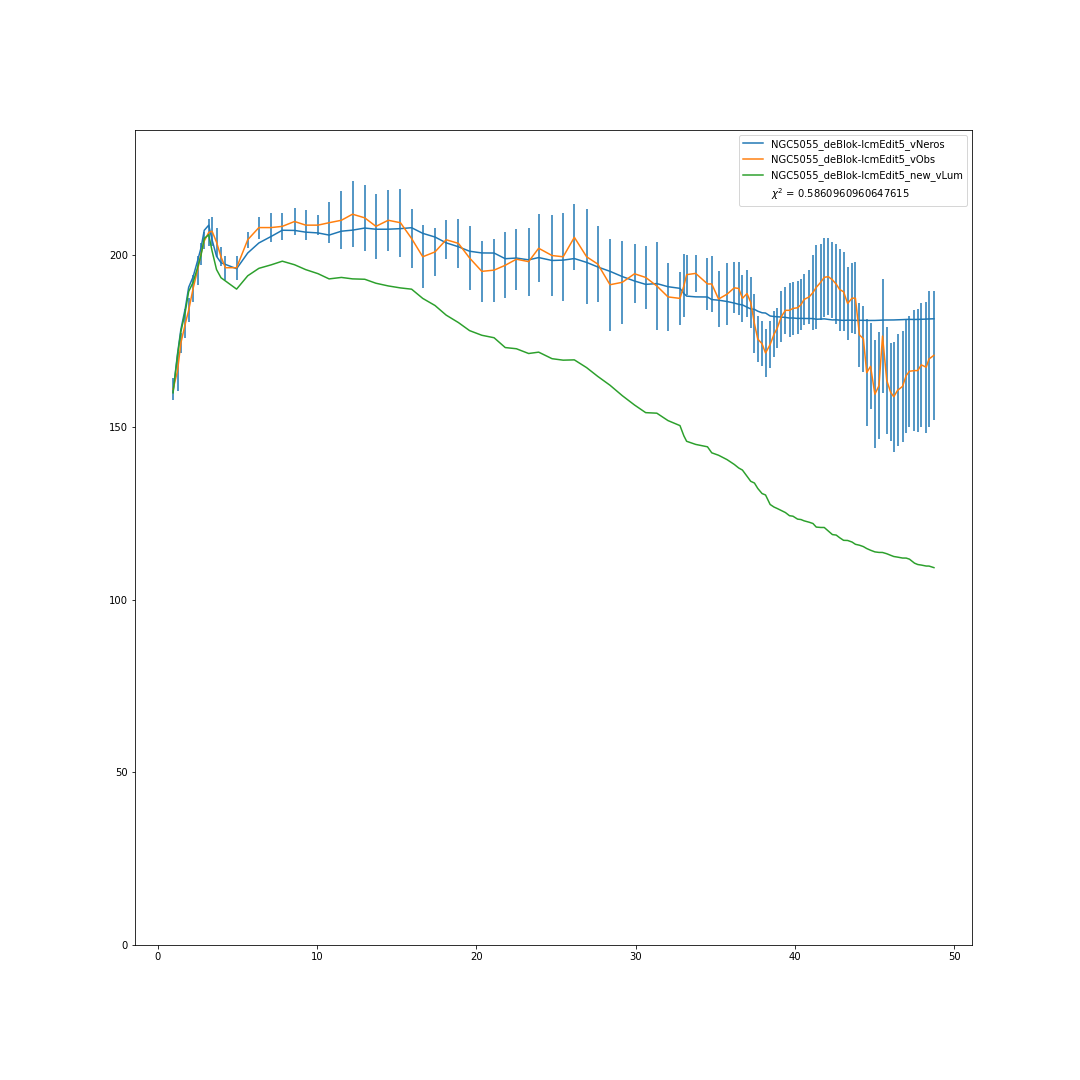
\includegraphics[width=.8\linewidth]{NGC5055_deBlok-lcmEdit5_XueSofue}
  \caption{Lum edits5 \cite{Blok1}}
  \label{fig:sfig3}
\end{subfigure}
\caption{RCFM fits of NGC 5055 }
\label{fig:fig5055}
\end{figure}
 
 
 
  \begin{figure}[h]
\begin{subfigure}{.5\textwidth}
  \centering
  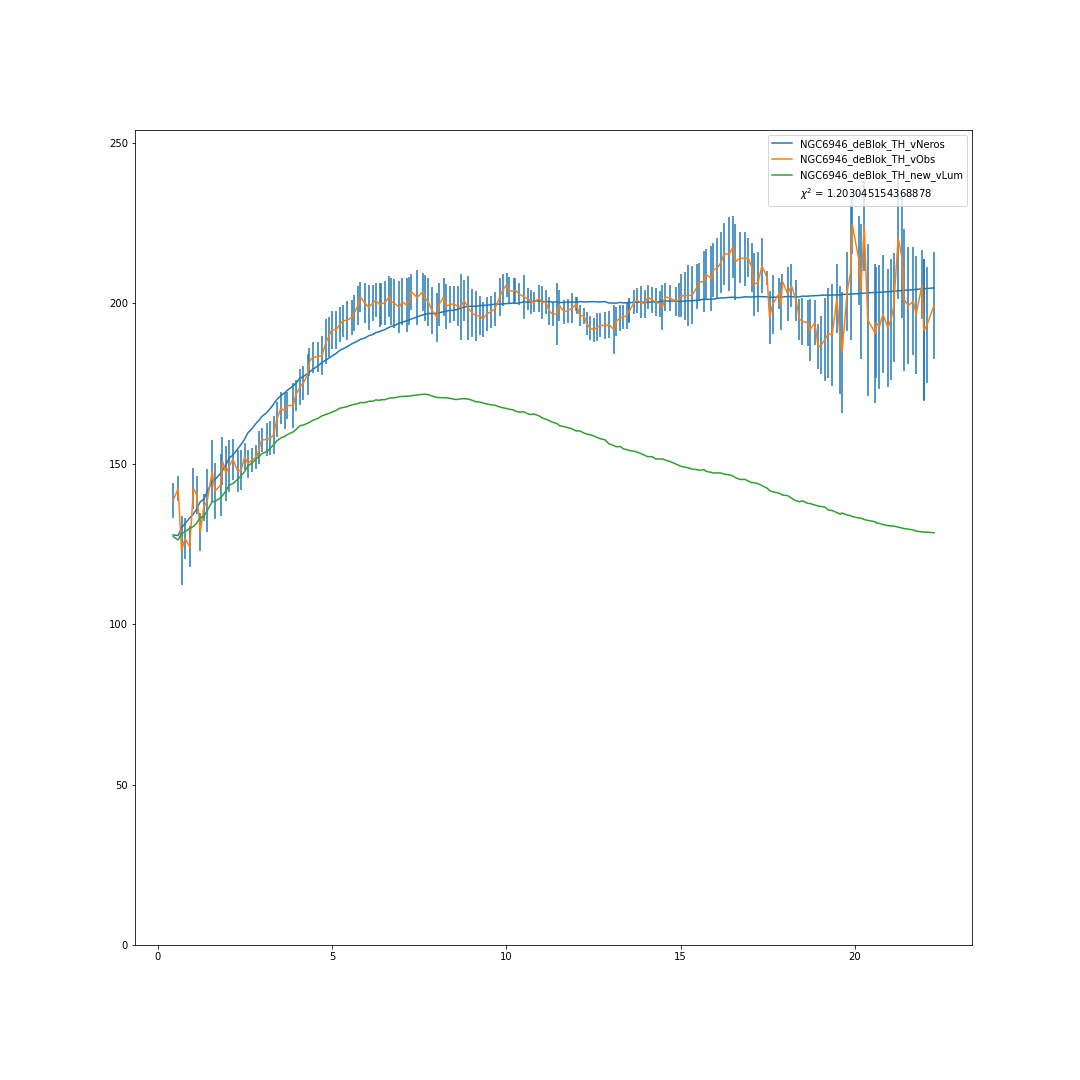
\includegraphics[width=.8\linewidth]{NGC6946_deBlok_TH_XueSofue}
  \caption{deBlok\cite{Blok1}}
  \label{fig:sfig4}
\end{subfigure}%
\begin{subfigure}{.5\textwidth}
  \centering
  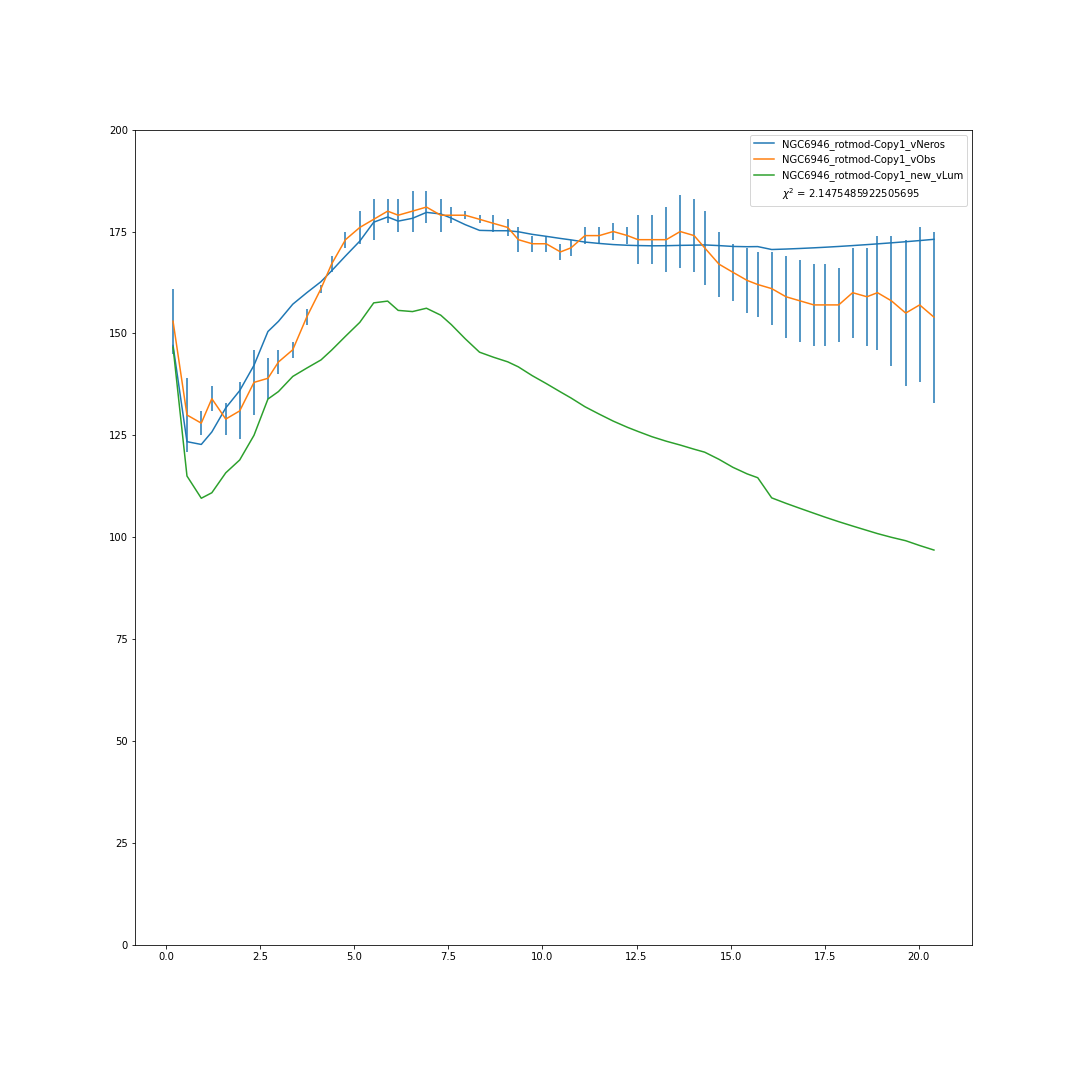
\includegraphics[width=.8\linewidth]{NGC6946_rotmod-Copy1_XueSofue}
  \caption{SPARC\cite{2016Lelli}}
  \label{fig:sfig5}
\end{subfigure}
\caption{RCFM fits  of NGC 6946 }
\label{fig:fig6946}
\end{figure}
%
%
%

  \begin{figure}[h]
\begin{subfigure}{.5\textwidth}
  \centering
  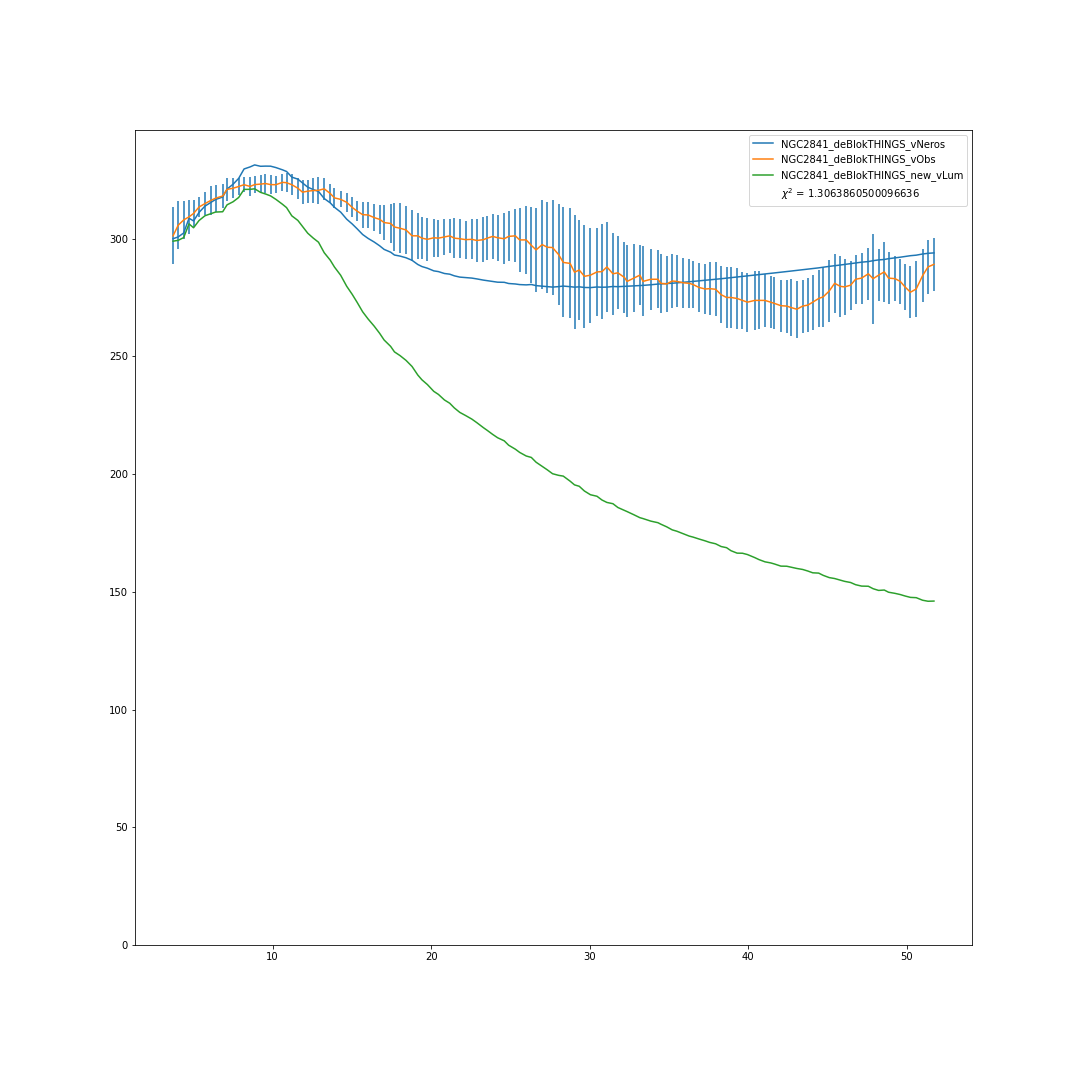
\includegraphics[width=.8\linewidth]{NGC2841_deBlokTHINGS_XueSofue}
  \caption{deBlok\cite{Blok1}}
  \label{fig:sfig9}
\end{subfigure}%
\begin{subfigure}{.5\textwidth}
  \centering
  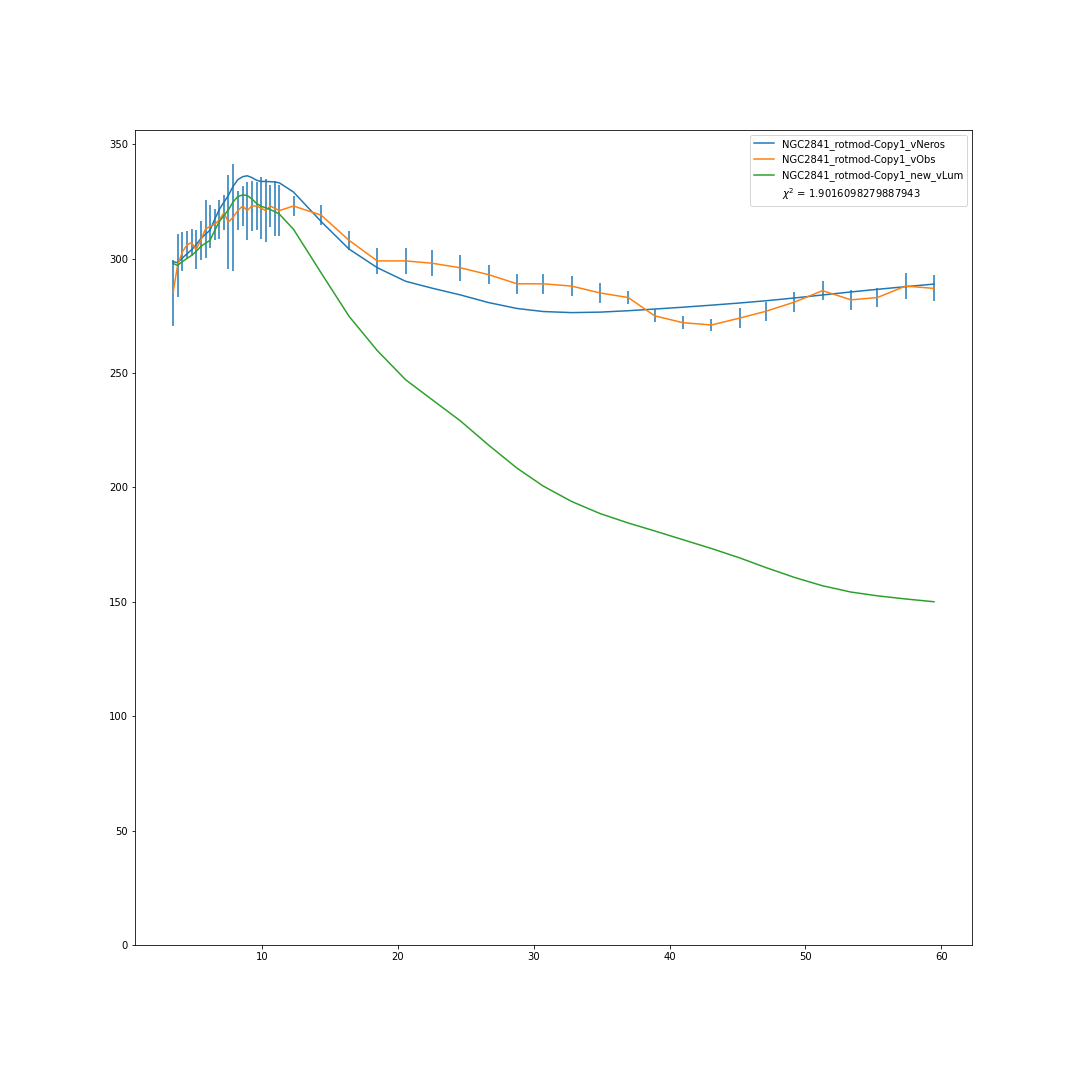
\includegraphics[width=.8\linewidth]{NGC2841_rotmod-Copy1_XueSofue}
  \caption{SPARC\cite{2016Lelli}}
  \label{fig:sfig10}
\end{subfigure}
\caption{RCFM fits  of NGC 2841}
\label{fig:fig2841}
\end{figure}

\clearpage
  \begin{figure}[h]
\begin{subfigure}{.5\textwidth}
  \centering
  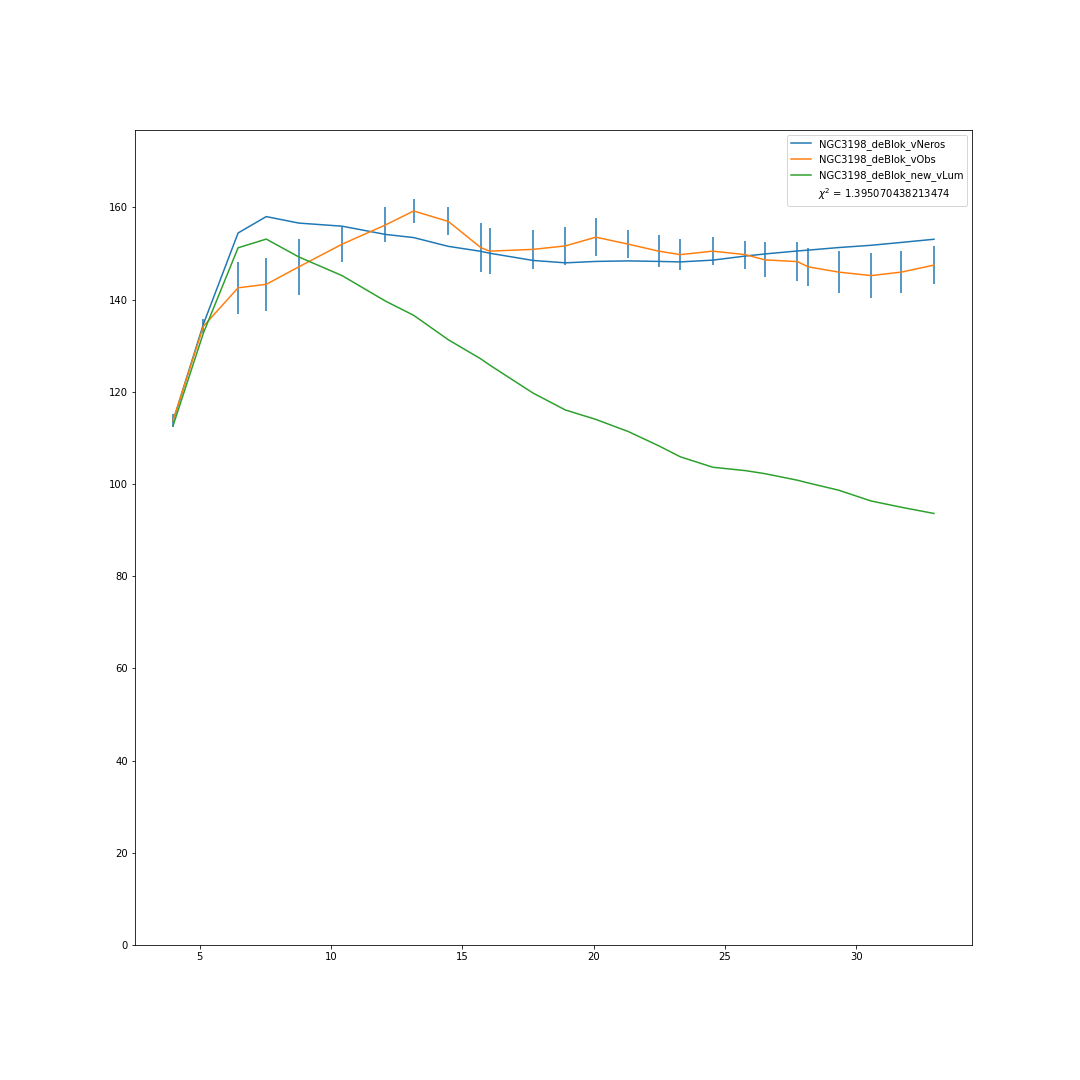
\includegraphics[width=.8\linewidth]{NGC3198_deBlok_XueSofue}
  \caption{deBlok \cite{Blok}}
  \label{fig:sfig6}
\end{subfigure}%
\begin{subfigure}{.5\textwidth}
  \centering
  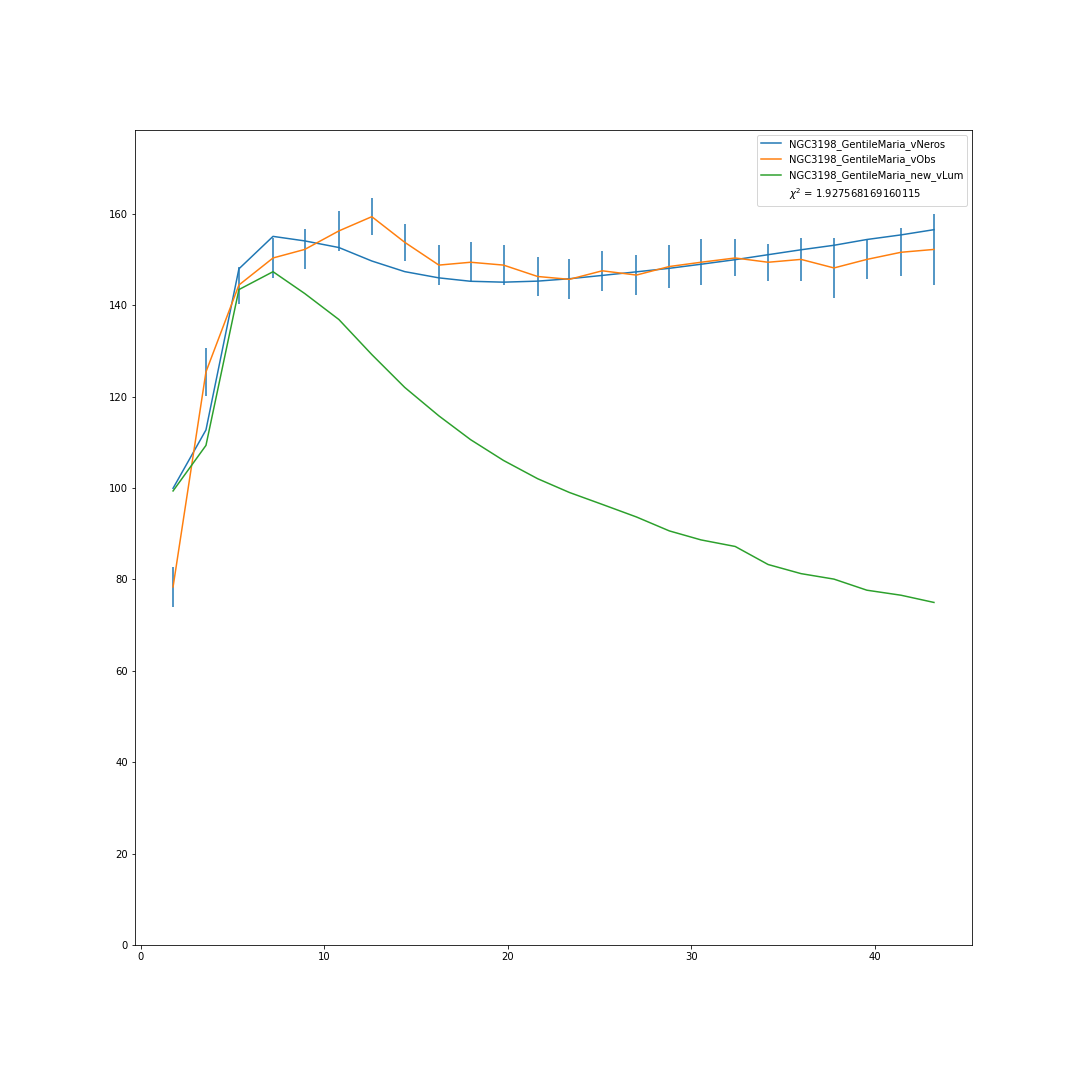
\includegraphics[width=.8\linewidth]{NGC3198_GentileMaria_XueSofue}
  \caption{Gentile \cite{Maria}}
  \label{fig:sfig7}
\end{subfigure}
\begin{subfigure}{.5\textwidth}
  \centering
  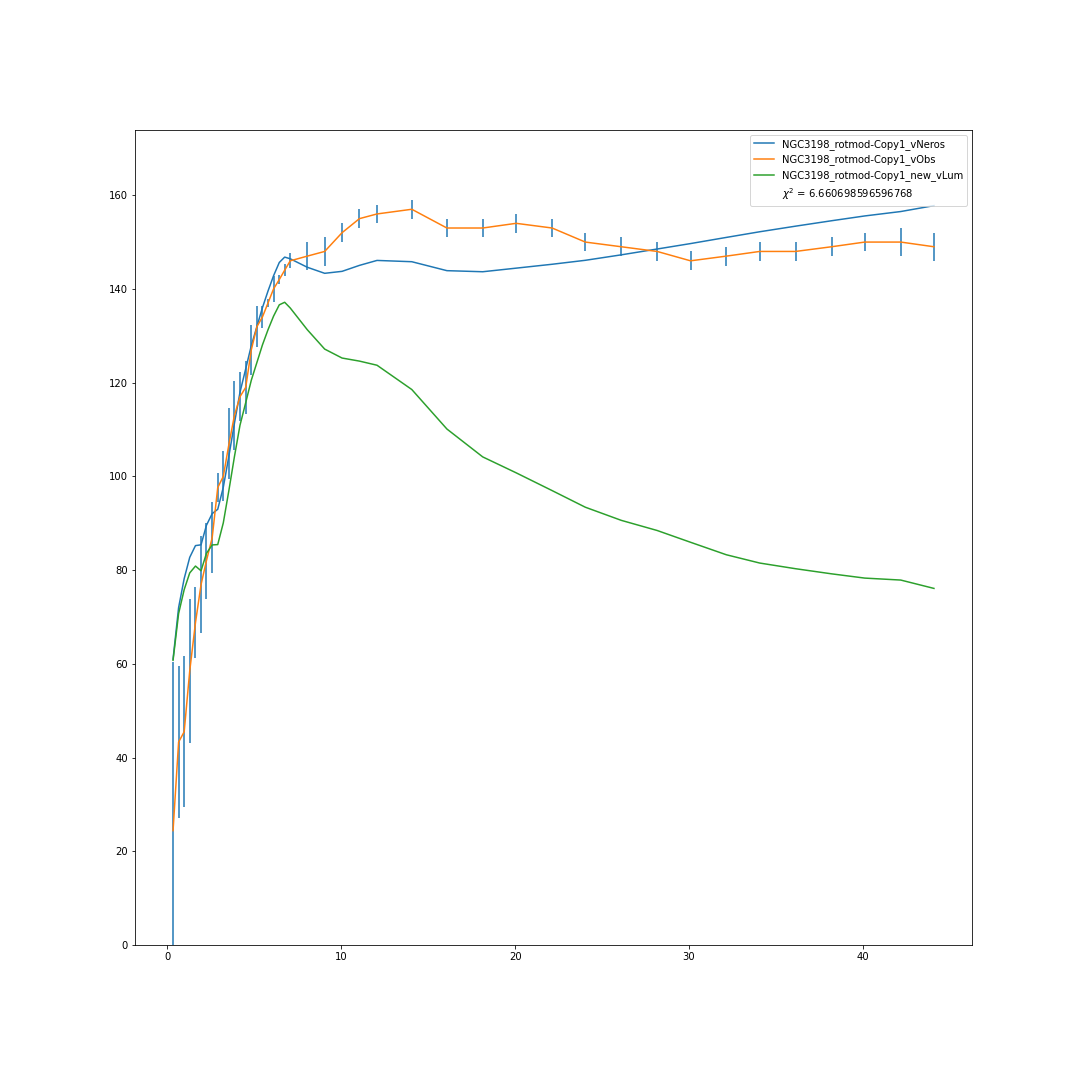
\includegraphics[width=.8\linewidth]{NGC3198_rotmod-Copy1_XueSofue}
  \caption{SPARC\cite{2016Lelli}}
  \label{fig:sfig8}
\end{subfigure}
\caption{RCFM fits  of NGC 3198}
\label{fig:fig3198}
\end{figure}
 %   
%
% 
\clearpage
%%%

  \begin{figure}[h]
\begin{subfigure}{.5\textwidth}
  \centering
  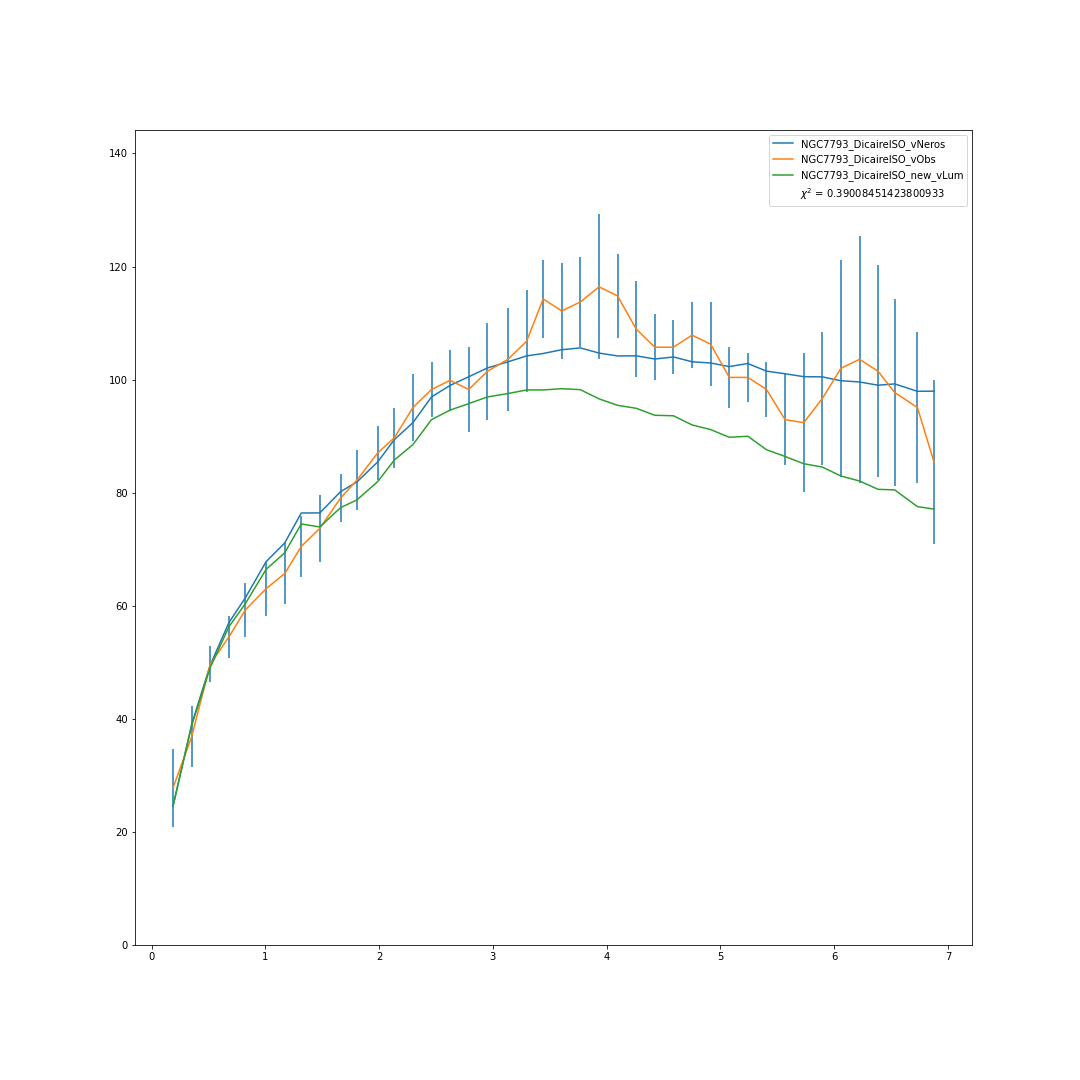
\includegraphics[width=.8\linewidth]{NGC7793_DicaireISO_XueSofue}
  \caption{Dicaire \cite{Dicaire1}}
  \label{fig:sfig11}
\end{subfigure}%
\begin{subfigure}{.5\textwidth}
  \centering
  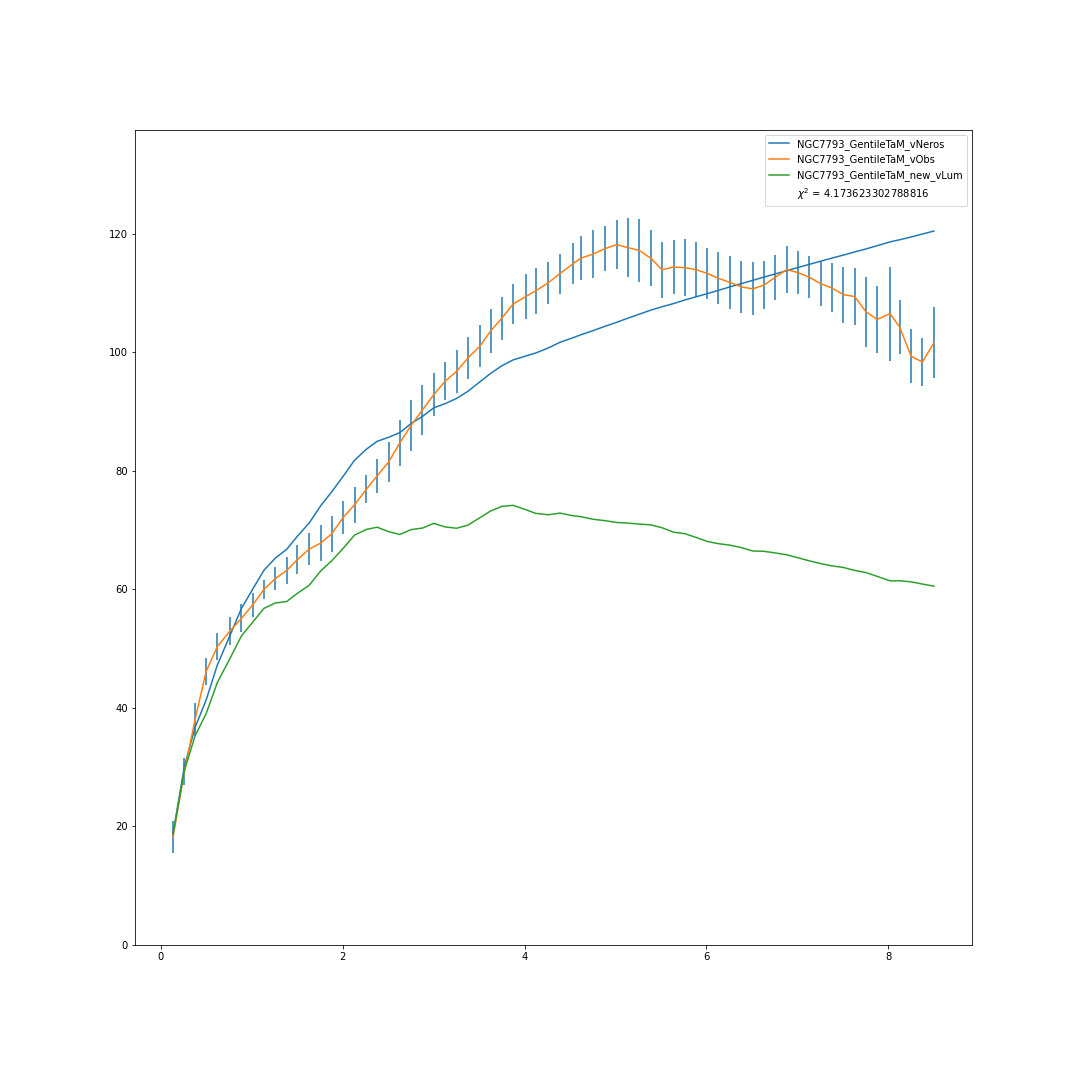
\includegraphics[width=.8\linewidth]{NGC7793_GentileTaM_XueSofue}
  \caption{Gentile\cite{Gent}}
  \label{fig:sfig12}
\end{subfigure}
\begin{subfigure}{.5\textwidth}
  \centering
  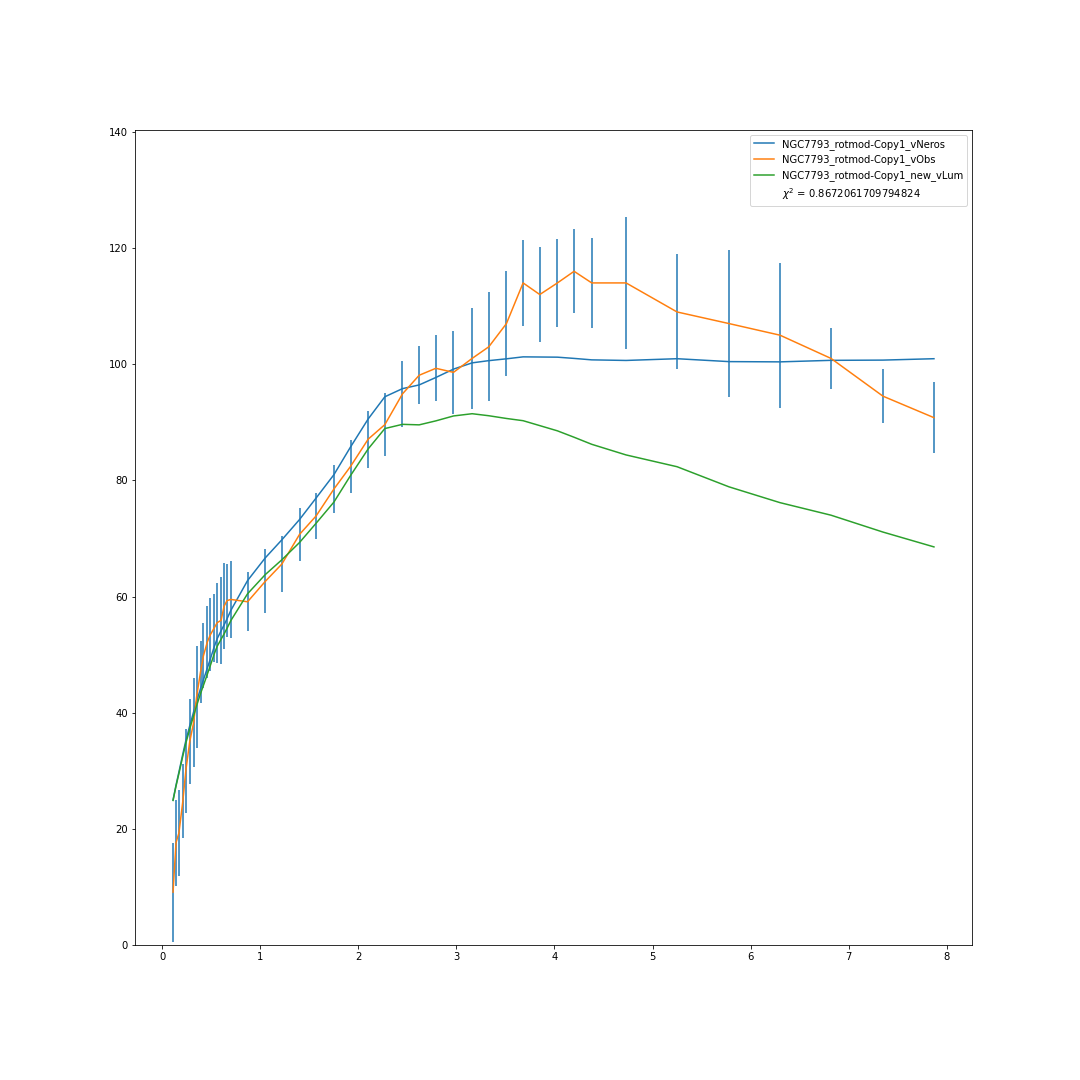
\includegraphics[width=.8\linewidth]{NGC7793_rotmod-Copy1_XueSofue}
  \caption{SPARC\cite{2016Lelli}}
  \label{fig:sfig13}
\end{subfigure}
\caption{RCFM fits  of NGC 7793}
\label{fig:fig7793}
\end{figure}
%
%
%
%
\clearpage
  \begin{figure}[h]
\begin{subfigure}{.5\textwidth}
  \centering
  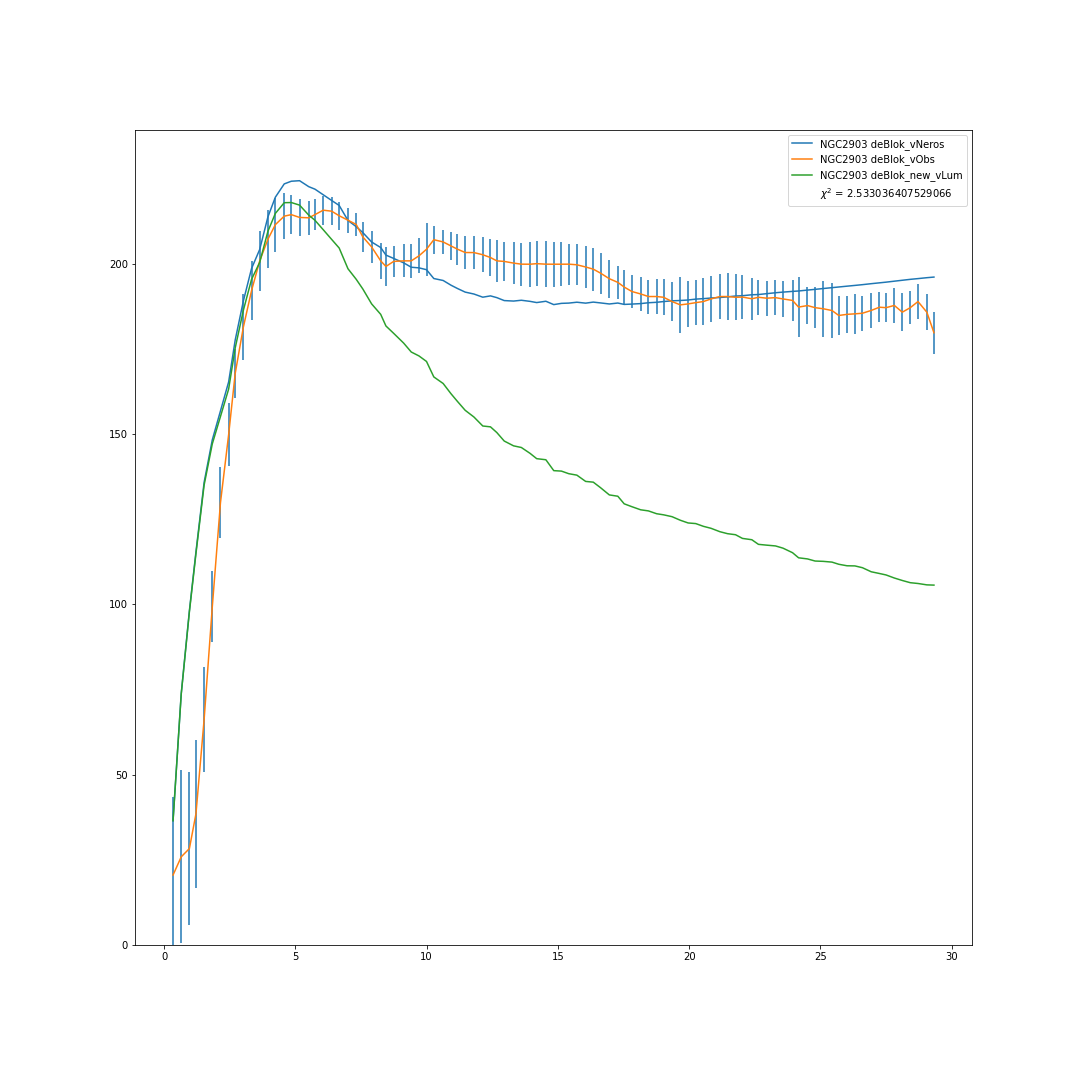
\includegraphics[width=.8\linewidth]{NGC2903deBlok_XueSofue.png}
  \caption{deBlok\cite{Blok1}}
  \label{fig:sfig14}
\end{subfigure}%
\begin{subfigure}{.5\textwidth}
  \centering
  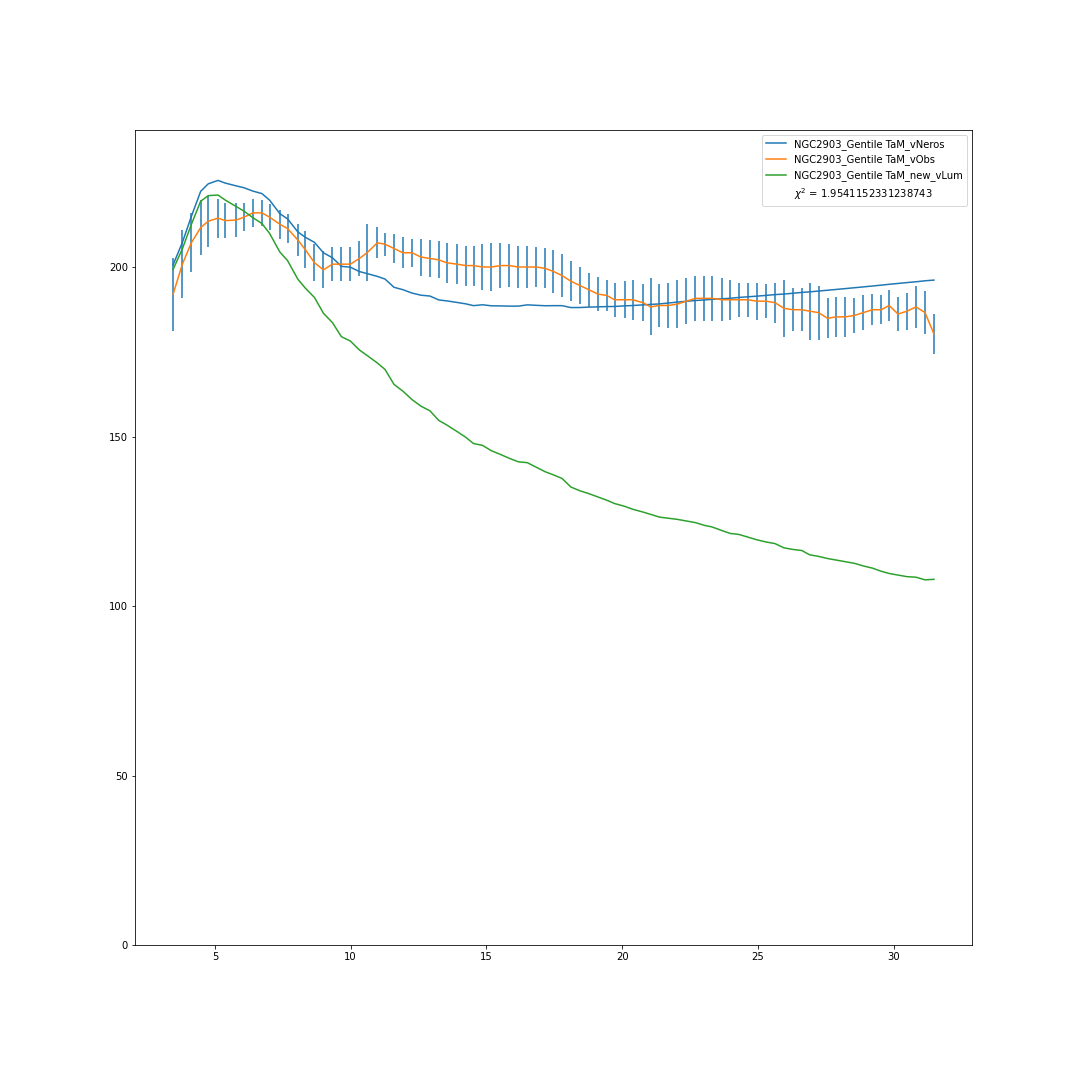
\includegraphics[width=.8\linewidth]{NGC2903_GentileTaM_XueSofue.png}
  \caption{Gentile\cite{Gent}}
  \label{fig:sfig15}
\end{subfigure}
\begin{subfigure}{.5\textwidth}
  \centering
  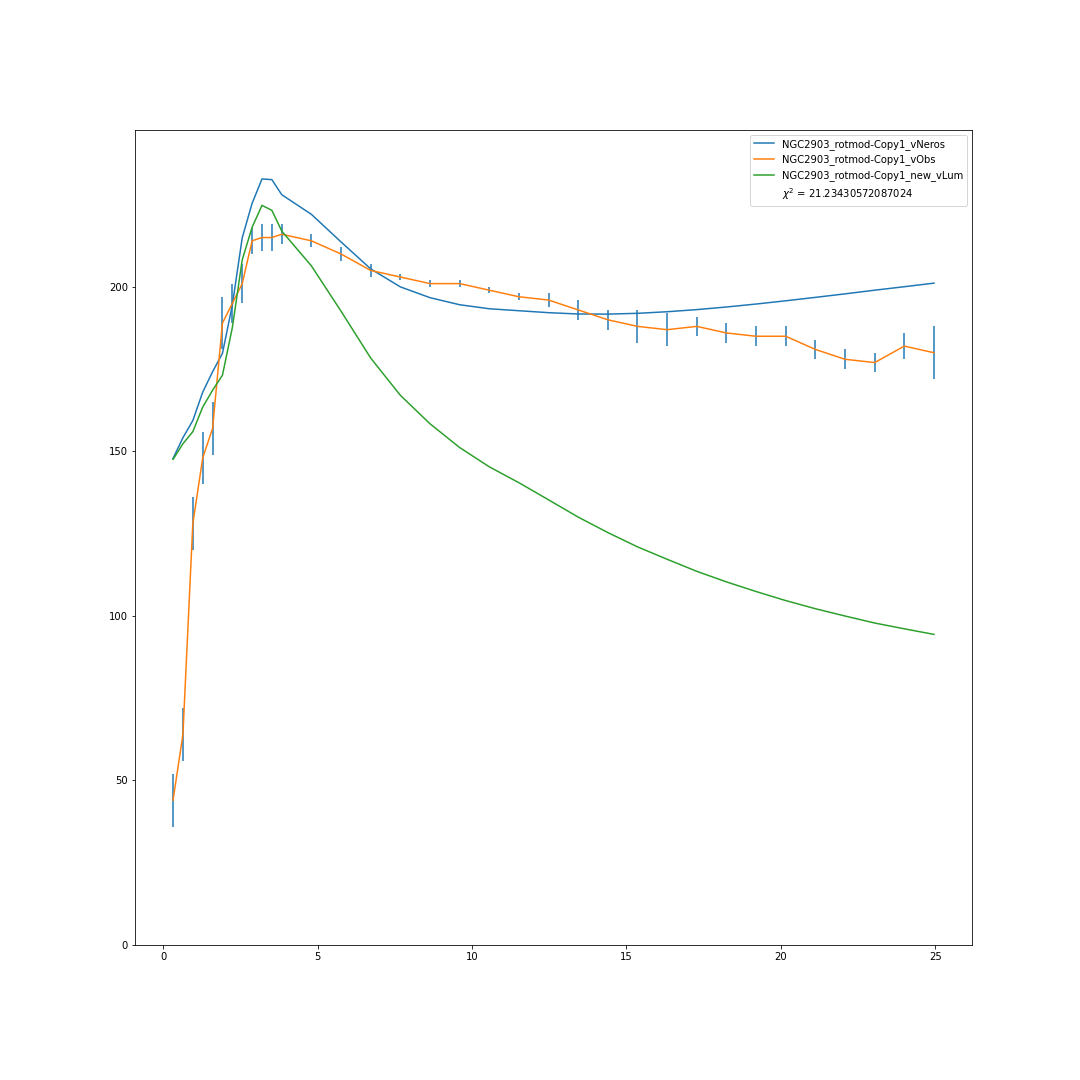
\includegraphics[width=.8\linewidth]{NGC2903_rotmod-Copy1_XueSofue.png}
  \caption{SPARC\cite{2016Lelli}}
  \label{fig:sfig16}
\end{subfigure}
\caption{plots of NGC 2903}
\label{fig:fig2903}
\end{figure}
%
\clearpage
%
%  
  \begin{figure}[h]
\begin{subfigure}{.5\textwidth}
  \centering
  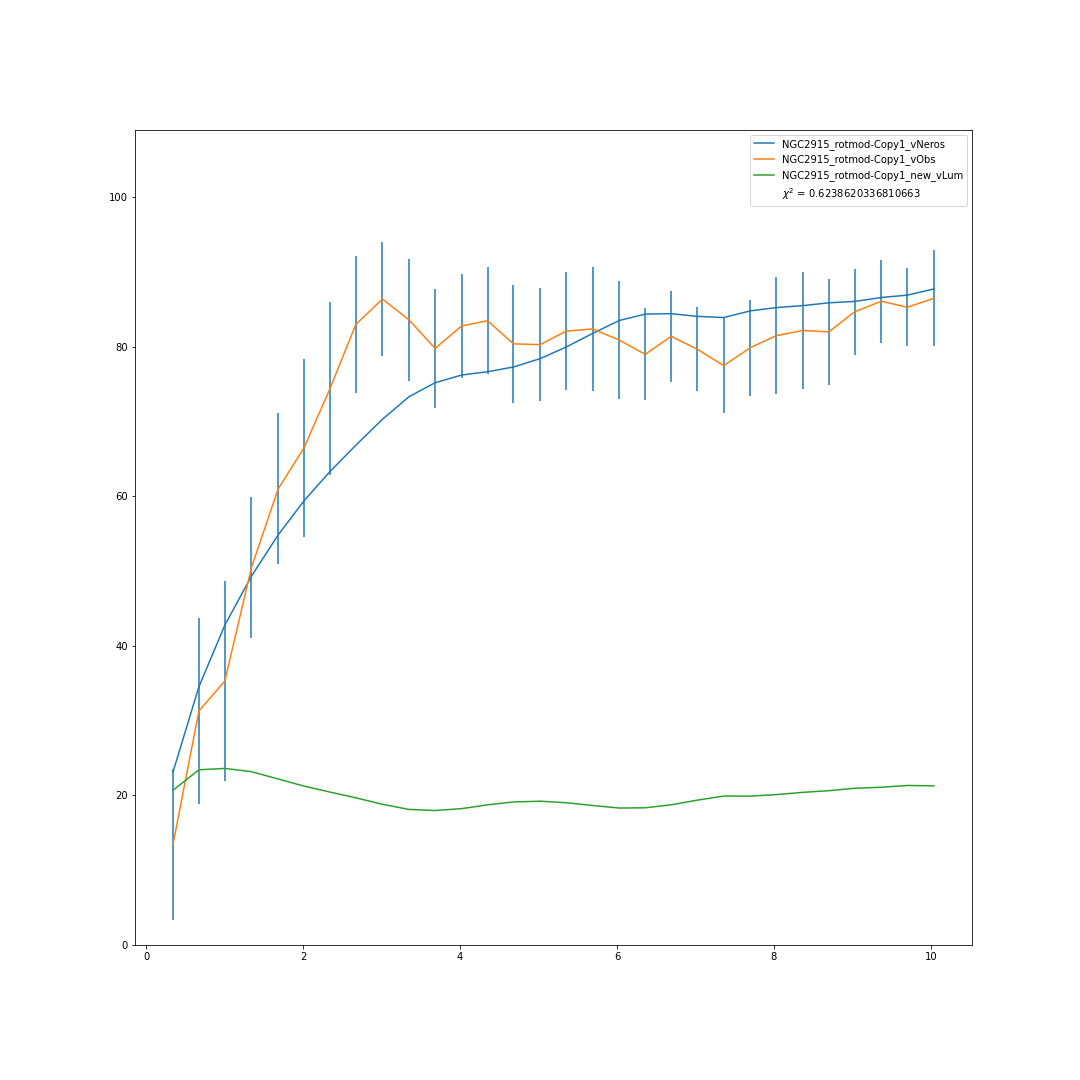
\includegraphics[width=.8\linewidth]{NGC2915_rotmod-Copy1_XueSofue.png}
  \caption{SPARC\cite{2016Lelli}}
  \label{fig:sfig17}
\end{subfigure}%
\begin{subfigure}{.5\textwidth}
  \centering
  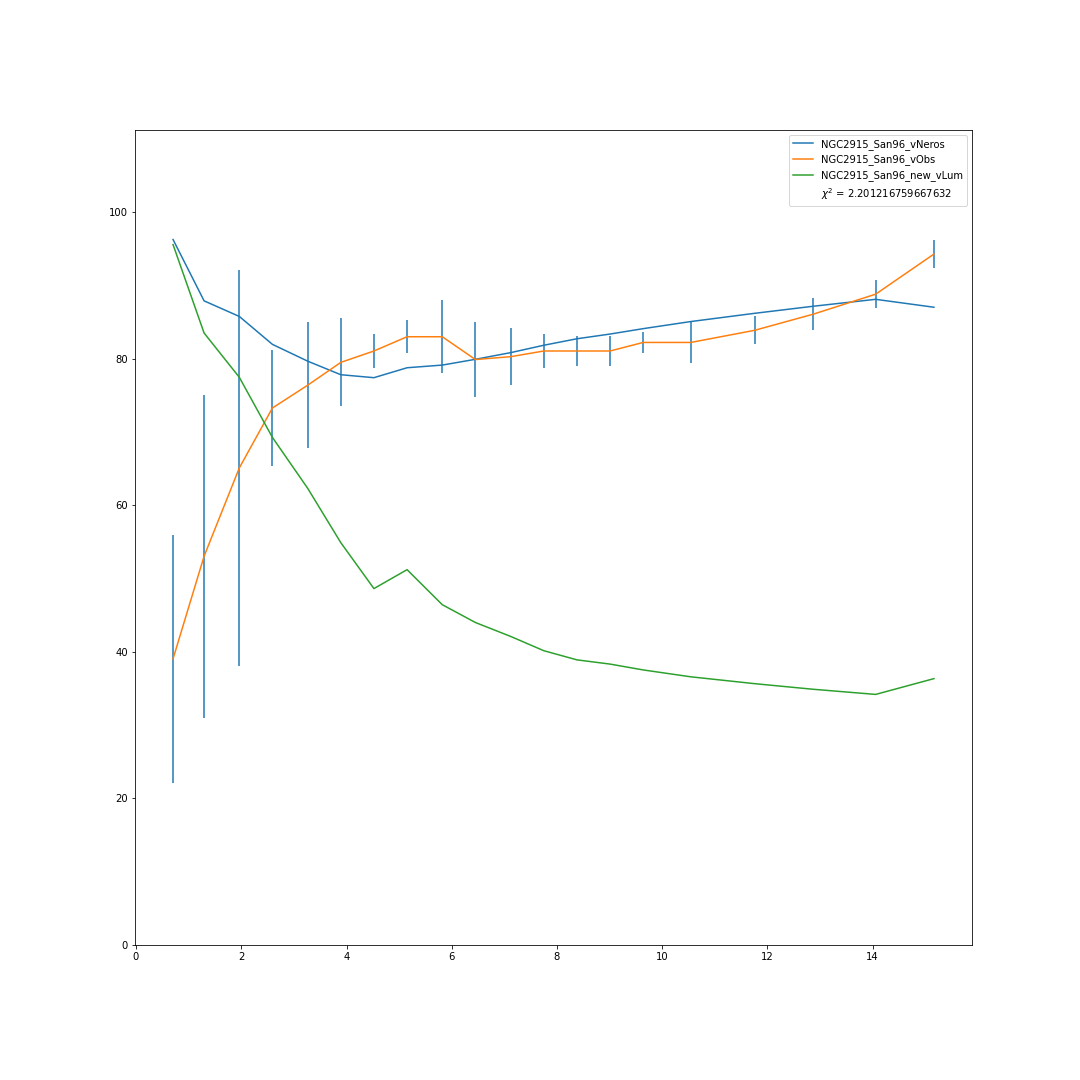
\includegraphics[width=.8\linewidth]{NGC2915_San96_XueSofue.png}
  \caption{Sanders\cite{San96}}
  \label{fig:sfig18}
\end{subfigure}
\caption{plots of NGC 2915}
\label{fig:fig2915}
\end{figure}
%
%
%
%  
%%%%%%%
  \begin{figure}[h]
\begin{subfigure}{.5\textwidth}
  \centering
  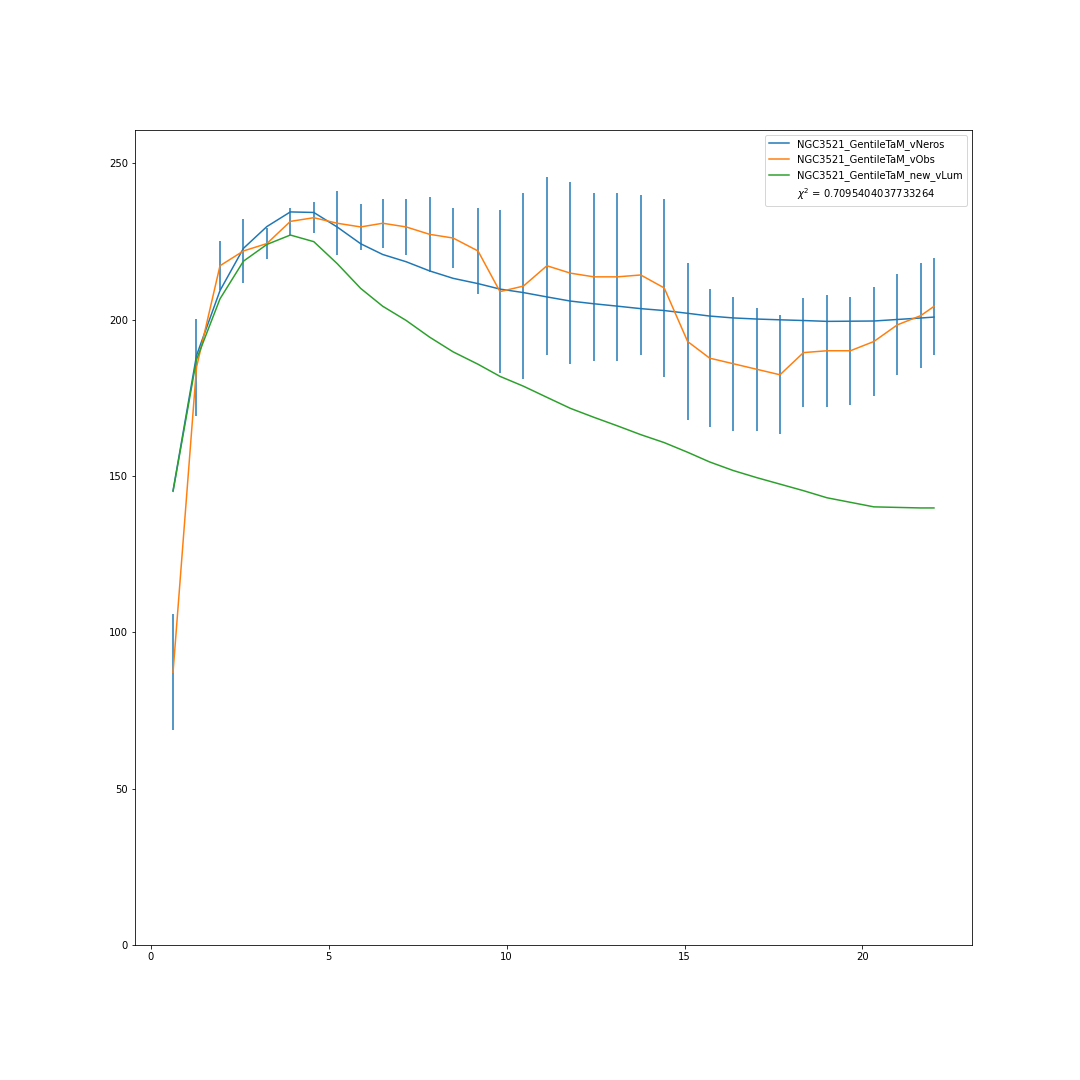
\includegraphics[width=.8\linewidth]{NGC3521_GentileTaM_XueSofue.png}
  \caption{Gentile\cite{Gent}}
  \label{fig:sfig19}
\end{subfigure}%
\begin{subfigure}{.5\textwidth}
  \centering
  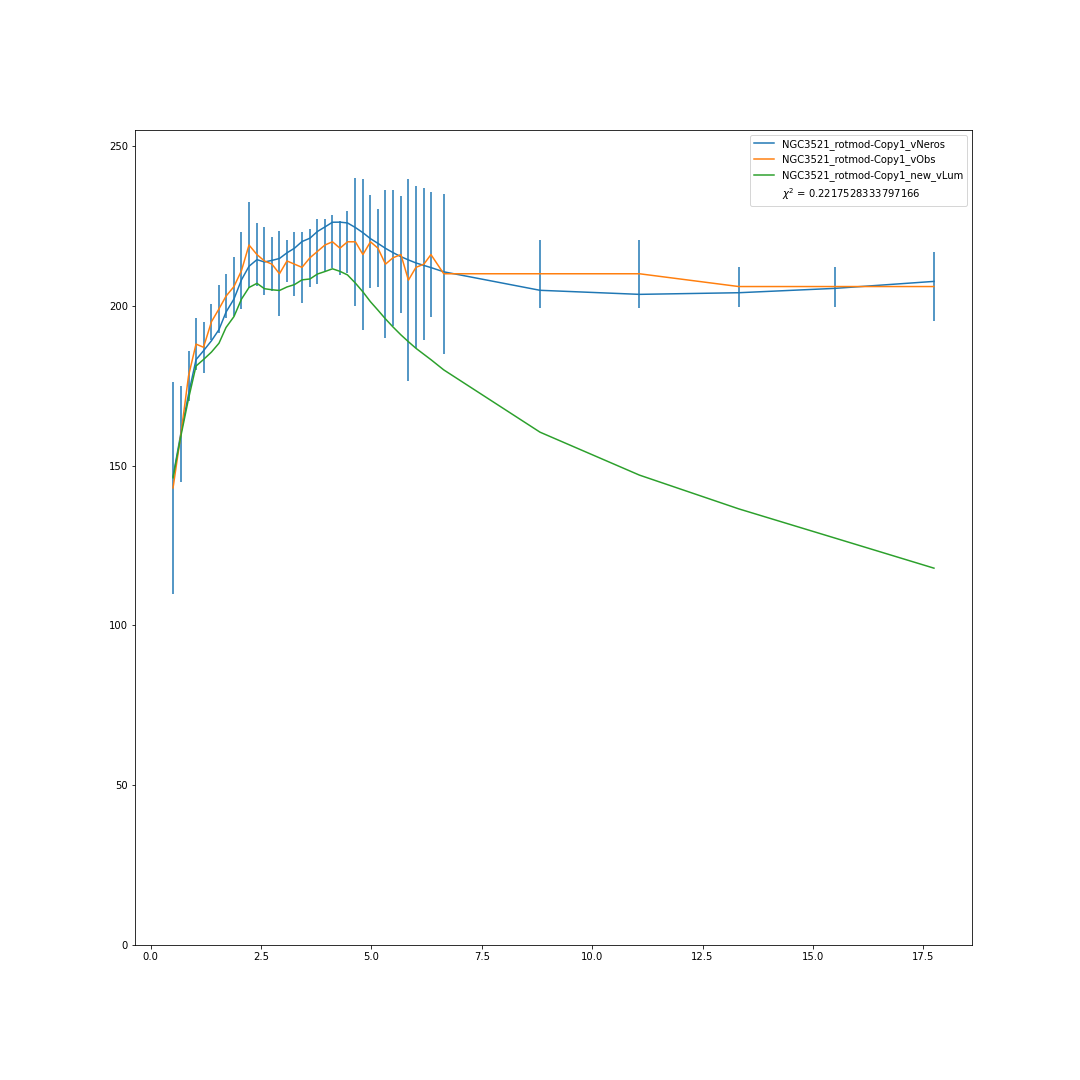
\includegraphics[width=.8\linewidth]{NGC3521_rotmod-Copy1_XueSofue.png}
  \caption{SPARC\cite{2016Lelli}}
  \label{fig:sfig20}
\end{subfigure}
\caption{plots of NGC 3521}
\label{fig:fig3521}
\end{figure}
%
%
%
\clearpage
 \begin{figure}[h]
\begin{subfigure}{.5\textwidth}
  \centering
  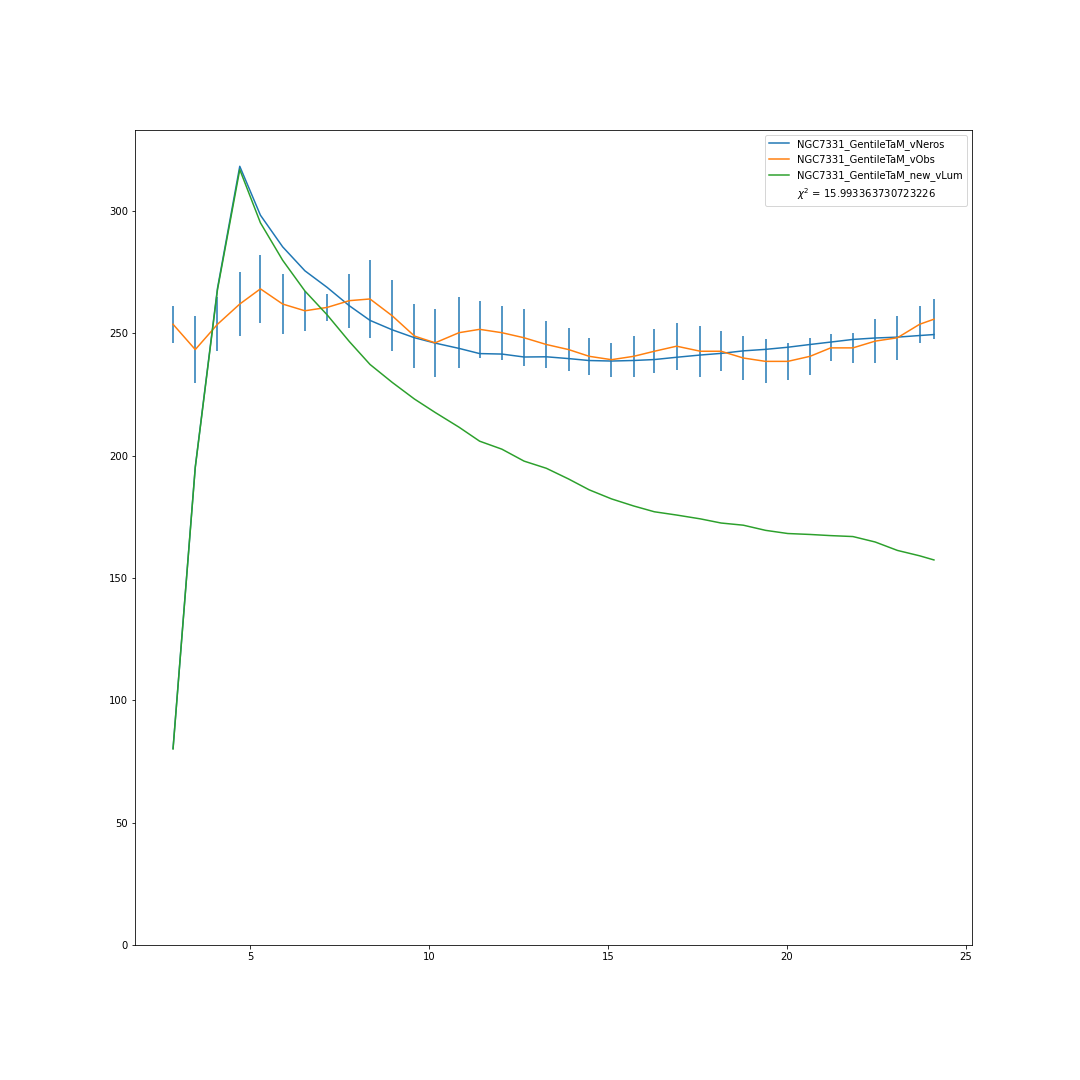
\includegraphics[width=.8\linewidth]{NGC7331_GentileTaM_XueSofue.png}
  \caption{Gentile\cite{Gent}}
  \label{fig:sfig21}
\end{subfigure}%
\begin{subfigure}{.5\textwidth}
  \centering
  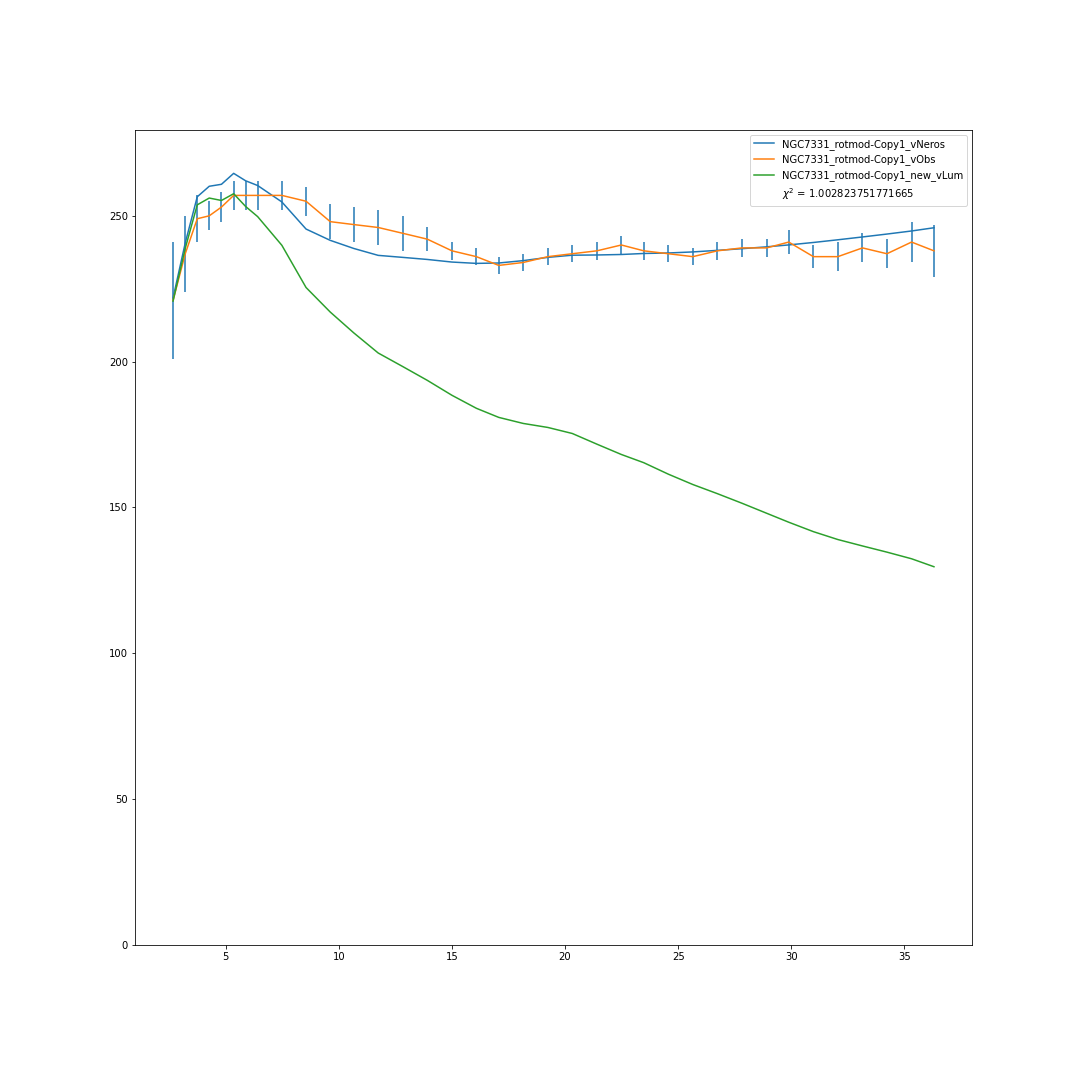
\includegraphics[width=.8\linewidth]{NGC7331_rotmod-Copy1_XueSofue.png}
  \caption{SPARC\cite{2016Lelli}}
  \label{fig:sfig22}
\end{subfigure}
\caption{plots of NGC 7331}
\label{fig:fig7331}
\end{figure}
%%%%%%%
 \begin{figure}[h]
\begin{subfigure}{.5\textwidth}
  \centering
  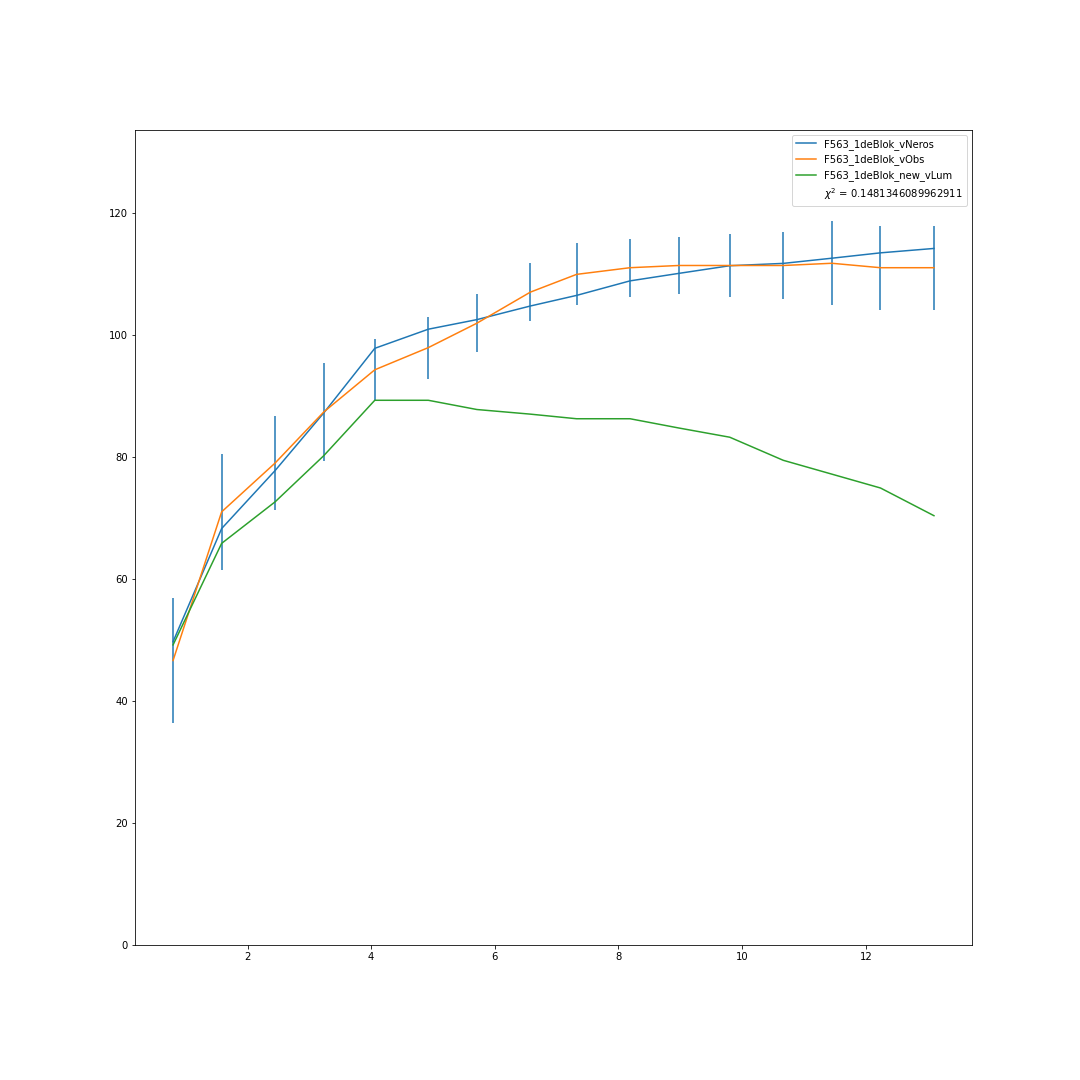
\includegraphics[width=.8\linewidth]{F563_1deBlok_XueSofue.png}
  \caption{de Blok}
  \label{fig:sfig23}
\end{subfigure}%
\begin{subfigure}{.5\textwidth}
  \centering
  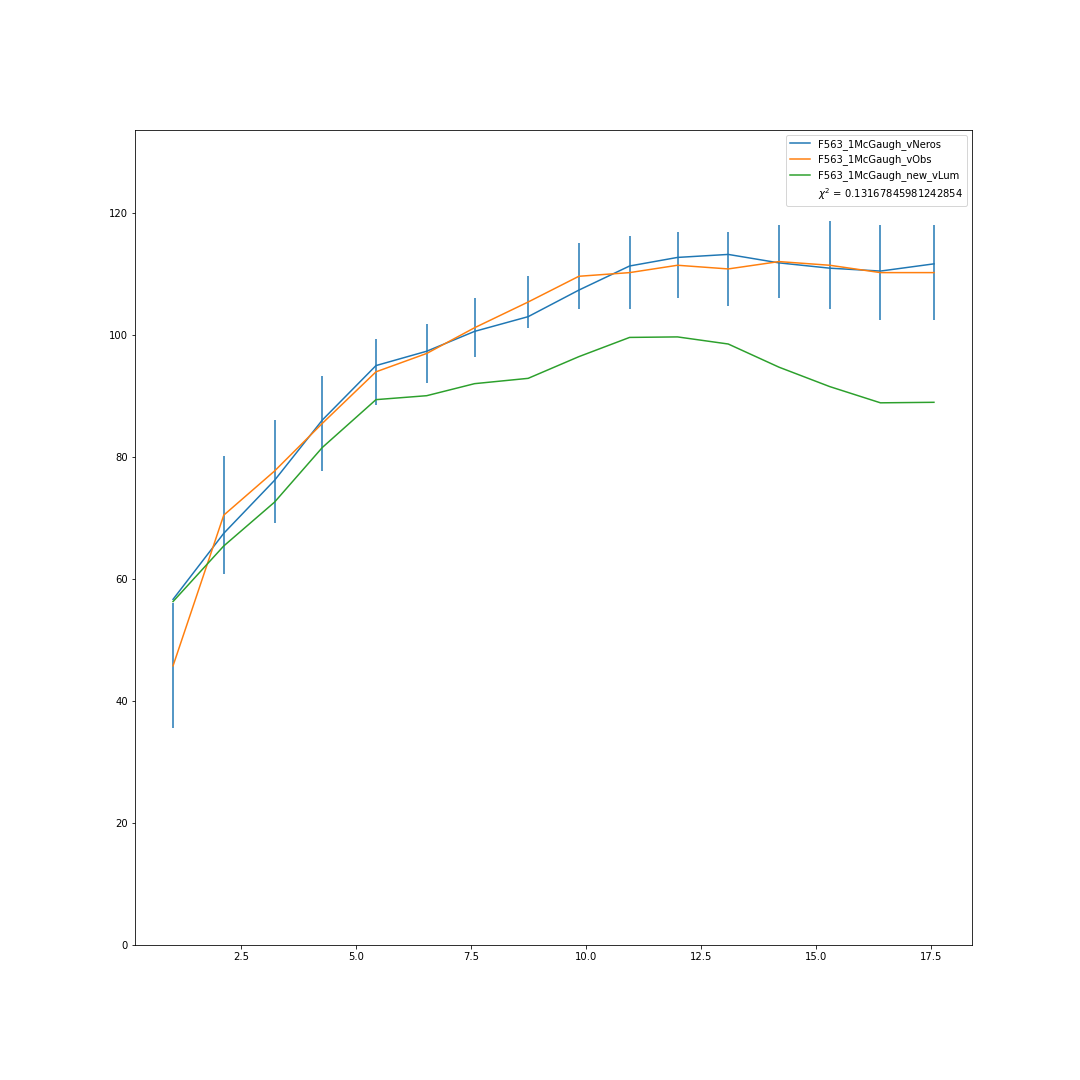
\includegraphics[width=.8\linewidth]{F563_1McGaugh_XueSofue.png}
  \caption{McGaugh}
  \label{fig:sfig24}
\end{subfigure}
\caption{plots of F563-1}
\label{fig:figF563-1}
\end{figure}
\clearpage
%%%%%%
%%%%%%%%
%%%%%%
%%%%%%%
%%%%%%
%%%%%%
\subsection{  free parameter and a ratio of luminosity to scale-length}
 
  
Estimates of luminous mass  (green line in Fig.\ref{fig:NGC2403})   are   considered Lorentz scalars, 
and Doppler shifted spectra (blue line in Fig.\ref{fig:NGC2403})  are considered as components of 4-vectors. Lorentz scalars  are agreed upon between frames, given a reliable distance estimate, so we   fix our model's free parameter on a SPARC subset where distances are measured by either   Cepheids and Tip of the Red Giant Branch (CITE McGaugh)).  
 

 We show a significant  correlation between the free parameter and the ratio of total light $L$ to the effective scale-length $gradient in that light$. 
 
 
 %%%%%%
%%%%%%%%
%%%%%%
%%%%%%%
%%%%%%
%%%%%%

 
   
 
 
 
 


 
  
  
 

 
% \cite{McGaugh2016RAR} is the other one. This one describes the sample. 175 SPARC galaxies. Describes all the assumptions for the disk, gas, bulge models, the band used and reasoning, rotation curve data from HI, 
 
% They only fit a subset (153 of 175) of these galaxies.I get 128, I guess I'm cutting endpoints of 85 and 30 and they include. Plus I exclude like five that I think fail to fit
 
   
 
 
    
To fix the free parameter $\alpha$ in  our fitting formula in Eq.~\ref{eq:zonteLCM}, we exclude galaxies with inclinations less than $30^o$ and more than $85^o$ from the SPARC sample due to uncertain kinematics and surface brightness measurements. This brings our sample from 174 to 131 galaxies of varying morphologies and surface brightnesses \cite{2016Lelli} that   we fit free.

 We find that the ratio of the total luminosity $L_{total}$ to    the half-light radius $R_{eff}$ \cite{Lelli_2016surface},  
 
 \begin{equation}
     \rho = L_{total}/R_{eff}
 \end{equation}
 
   is   strongly correlated with the $\alpha$. 
  
 \begin{figure}[h]
\scalebox{0.5}%
{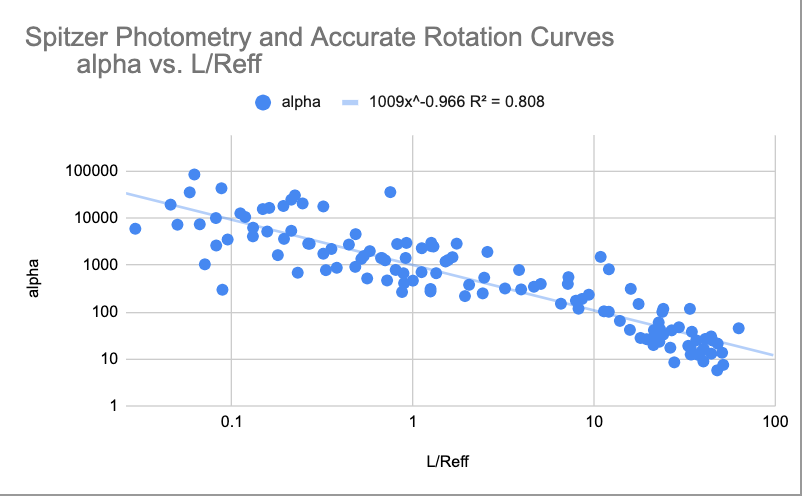
\includegraphics{alpha_9_29_21_minus3.png} }
\caption{ inverse frame order and   anomalous sign }
\label{alpha2}
\end{figure}  

 \begin{figure}[h]
\scalebox{0.5}%
{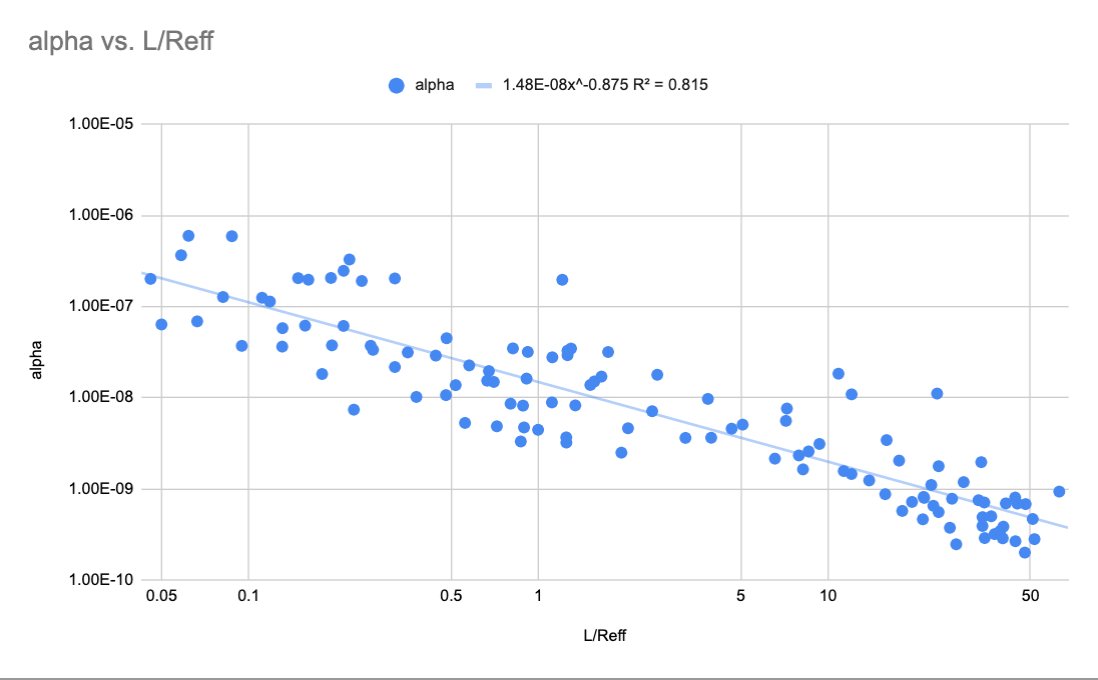
\includegraphics{sech1Coth2.png} }
\caption{   Function: sech1coth2. correct frame order. correct sign. }
\label{alpha3}
\end{figure} 


If we assume that $\alpha$ is a ratio of the same quantity for  the Milky Way $\rho_{mw}$ with respect to the other   galaxy $\rho_{gal}$  

\begin{equation}
\alpha=\left(\frac{\rho_{mw}}{\rho_{gal}}\right)^{b}  ,
\label{correl}
\end{equation}

then we arrive at a similar fit (See Fig.~\ref{alpha1}, here with six galaxies removed that seem to be local minima solutions).



\begin{figure}[h]
\scalebox{0.5}%
{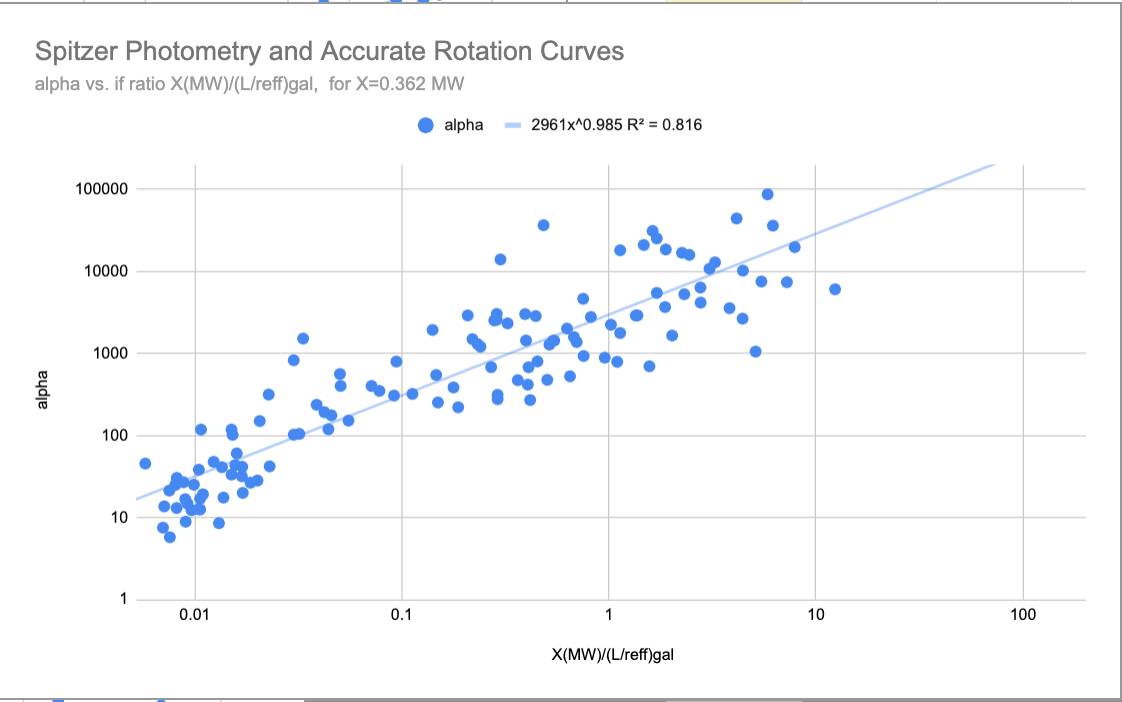
\includegraphics{alphaSept2021} }
\caption{ with MW in  numerator and minus six galaxies. Function with anomalous minus sign }
\label{alpha1}
\end{figure} 

 
  

 
  
 \section{  Conclusions   }
********
******

 
{   \color{teal} Everyone: add stuff here as you go.  }
{\color{red} This heuristic replacement of dark matter is not fundamental in nature, but    one supposes if it is possible to quantify these
excesses in shifted spectra using entirely luminous mass as we do in this paper,  then a   fundamental derivation may exist.  The curious conspiracy of the luminous mass to   determine the dark matter  is here rephrased as a question of imprints on shifted spectra from our Milky Way.  This model has a static choice of the Milky Way, which is underdetermined, as well as a free parameter. We show in this paper a set of fits with the free parameter and Milky Way choices fixed. 
 }
 
 
 % \caption{Results   for SPARC Luminous mass profiles  [NOT UPDATED]\label{sumRESULTS}}
 % \begin{tabular}{@{}llccccccc@{}}
 % \hline
 %  Galaxy     	  &Ref.~&  \multicolumn{3}{c}{\underline{ Other Model Fit Results}}	& & \multicolumn{3}{c}{\underline{LCM Fit Results }}  \\
%\hline
%   	 	& & &  $M/L_{disk}$		& $\chi^2_r$	&&$M/L$&$r_e$&$\chi^2_r$ \\ 
% \hline
%F 563-1	& 2	%& 			
%					&NFW	&--	 		&-- & 	&1.13 	&2.84 	&0.06 \\
%M 31* 	& 12 	%&7.5
%					&ISO	 	 &7.50		&0.36 & 	&5.88	 &4.80 	&0.04  \\
%M 33		& 5	 %&	K 		
%					& NFW 	&0.70		&2.46&  	 &1.98	 &1.46	& 0.17 \\
%NGC 891*	& 11 	% &3.6$\,\umu$m 
		%			&MaxLight &0.9 			&1.10  & 	 &--  	 &	&0.25 \\ 
%NGC 925 	&3	%&3.6$\,\umu$m
 			%		&ISO 	&0.18		 &2.40& 	&0.92	 &4.35	&0.11 \\
%NGC 2403	 & 3	%& 3.6$\,\umu$m
		%			& NFW	&0.41 	 	&4.56& 	&1.12	 	&2.18		& 0.88 \\
%NGC 2841*  &6-3	% & 3.6$\,\umu$m
%					&  James	&0.74 	 	&0.45 & 	&6.25	  &4.84	&0.11 \\
%NGC 2903  &10	 %&B	   		
%					&MOND   	&3.60 	 	&10.71& 	 &2.2	 	&2.81		&0.47\\
% NGC 3198 & 3 	%&3.6$\,\umu$m
%					 &NFW	&0.80	   	&5.40  &   	 &1.80 	 &5.10	&0.64   \\
%NGC 3521  & 8-6	 %&3.6$\,\umu$m 
%					&MOND	&0.71 	 	&0.97 & 	 &2.13  &3.23	&0.22 \\
%NGC 3726	& 10	%&B 			
%					&MOND	&1.00	 	&3.57& 	&1.06	 &2.70	&0.05 \\
%NGC 3953	& 10	%&B 			
%					&MOND	&2.7		 	&1.35& 	&1.79 	&2.60 	&0.35 \\
%NGC 3992	& 10	%&B 			
%					&MOND	&4.93	 	&0.50& 	&2.45 	 &4.77	&0.04 \\
%NGC 4088	& 10	%&B 			
%					&MOND	&1.16		 	&1.70& 	&5.58	 &2.70	&0.27 \\
%NGC 4138	& 10	%&B 			
%					&MOND	&3.5		 	&2.12& 	&3.67	 &1.46	&0.01 \\
%NGC 5055*	 & 3	%&3.6$\,\umu$m 
%					&  NFW	&0.79	 	&17.23&  	&5.87	 &3.29	&0.69 \\
%NGC 5533*	 & 10 %&B 			
%					&MOND	&0.6		  	&1.57 & 	&7.11 	  &3.23	&0.22  \\
%NGC 5907*	& 10	%&B 			
				%	&MOND	&1.6 		 	 &0.44& 	&2.04	 &3.45	%&0.09 \\
%NGC 6946*	&  10	 %& B			
%					&  MOND	& 0.5		 	&   3.03& 	&1.44 	 &0.76	&0.07  \\ 
%NGC 6946*	&  3	 %& B			
%					&  NFW	& 0.5		 	&   3.03& 	&1.44 	 &0.76	&0.07  \\ 
%NGC 7331	&8	% & 3.6$\,\umu$m
%					&James	&0.4 		 	& 0.45& 	&1.34	 &2.44	&0.09 \\
%NGC 7793  &14	%&B			
%					&ISO		&2.6		 	&1.08& 	&2.7	 &1.51	&0.11 \\
%NGC 7814* &11 	% & 3.6$\,\umu$m
%					&ISO   	& 0.68  	 	& 0.25& 	 &-- 	   &	&0.20 \\ 
%UGC 128		&6	%&				
	%				&James	&			&	&	&1.58	  &10.3	%&0.20\\
%UGC 6973	& 10	%&B 			
%					&MOND	&2.7		 	&23.5 & 	&--  	& 	&0.06 \\
%UGC 7524	& 6	%&B 			
%					&James	&--		 	&-- & 	&2.10 	&3.32 	&0.06 \\
% 1.~\citet{Bege}, 2.~\citet{JNav}, 3.~\citet{Blok} , 4.~\citet{Maria}, 
%5.~\citet{Cor03}, 6.~\citet{James},   7.~\citet{Batt},   8.~\citet{Gent},   9.~\citet{Bot},   10.~\citet{SanMcGa},
 % 11.~\citet{Frat},   12.~\citet{Car},   13.~\citet{giraud2000universal},   14.~\citet{Dicaire}, %15.~\cite{Klypin}. \\
%    \end{minipage}
%\end{table*} 


   

  \section[]{Acknowledgments}
 This work is dedicated to Emmett Till. This paper was completed with gratitude on the usual, accustomed, and unceded territories
of the Cheyenne, Arapaho and Ute Tribal Peoples.
  The authors would like to thank  V.\,P.\,  Nair,   R.\, Walterbos, S.\ McGaugh, A.\, Klypin, K. Bender, C. Beetle and     T.\, Boyer.   \\
  
 
%The   dark matter problem  is currently woven into most faces of our cosmology (weaklensing, galaxy rotation curves, early structure formation, galaxy and cluster interactions).   We posit that not all of these problems are actually the same physics problem.  We will address in this paper only the dark matter problem in spiral galaxies, the so-called flat-rotation curve problem discovered by \citet{1978Rubin,Bosma78}. We believe the ideas presented here are extensible to the problem of galaxy and cluster interactions, and perhaps weak lensing, but not to early structure formation, which we believe to be a different physics problem. 


 \appendix
 \begin{table*}[h!]
    \centering
    \begin{tabular}{|c|c|c|}
    Function $v_1  $ & $v_2$ & average $\chi^2_{ave}$ \\
    \hline \\
       $\left[ 1 -\frac{1}{\cosh {\gamma} } \right]  $ & $\coth \xi$ &\\
       \hline \\
       $ \frac{1}{\cosh {\gamma}}  $& &
       \hline \\
    \end{tabular}
    \caption{ {\color{red}make better TABLE of viable functions }

  The  best fit Lorentz-type mapping function for $(v1)$,  composed of the Lorentz exponential in  Eq.~\ref{eq:gravRS},}
    \label{tab:my_label}
\end{table*}
{\color{pink} \rule{\linewidth}{0.5mm}}

 
 
    
     

\bibliography{LCM} 

\end{document}
%
% ****** End of file apssamp.tex ******